\documentclass[12pt,oneside]{report}

% ---------- Gói lệnh ----------
\usepackage[T5,T1]{fontenc}
\usepackage[utf8]{inputenc}
\usepackage[utf8]{vntex}
\usepackage[a4paper,margin=2.5cm]{geometry}
\usepackage{graphicx}
\usepackage{amsmath,amssymb}
\usepackage{booktabs}
\usepackage{float}
\usepackage{caption}
\usepackage{subcaption}
\usepackage{tikz}
\usetikzlibrary{arrows.meta,positioning,calc,shapes.geometric,fit,backgrounds}
\usepackage{hyperref}
\hypersetup{colorlinks=true, linkcolor=black, citecolor=black, urlcolor=blue}

\renewcommand{\arraystretch}{1.15}

\tikzset{
  gatebox/.style={draw, rounded corners=2pt, minimum width=0.8cm, minimum height=0.7cm, fill=orange!25, font=\small},
  tanhbox/.style={draw, rounded corners=2pt, minimum width=0.8cm, minimum height=0.7cm, fill=blue!15, font=\small},
  opnode/.style={draw, circle, minimum size=0.42cm, inner sep=0pt, font=\footnotesize},
  dotn/.style={draw, circle, fill=black, minimum size=2.5pt, inner sep=0pt},
  cline/.style={-{Latex[length=2mm]}, thick},
  realcell/.style={draw, minimum width=0.8cm, minimum height=0.7cm, fill=blue!20, font=\scriptsize},
  predcell/.style={draw, minimum width=0.8cm, minimum height=0.7cm, fill=orange!35, font=\scriptsize},
  grubox/.style={draw, rounded corners=2pt, minimum width=1.1cm, minimum height=0.7cm, fill=green!15, font=\small},
}

\begin{document}

% ==================== TRANG BÌA ====================
\begin{titlepage}
\begin{center}


\includegraphics[width=3.2cm]{figures/logo.png}\\[0.4cm]
{\large\bfseries TRƯỜNG ĐẠI HỌC QUY NHƠN}\\[1.2cm]

{\Large\bfseries TIỂU LUẬN HỌC PHẦN}\\[0.3cm]
{\Large\bfseries HỌC SÂU VÀ ỨNG DỤNG}\\[0.5cm]
\rule{0.85\textwidth}{0.5pt}\\[0.8cm]

{\LARGE\bfseries ỨNG DỤNG MẠNG GRU DỰ BÁO NỒNG ĐỘ PM2.5\\[0.2cm] TẠI THÀNH PHỐ QUY NHƠN}\\[0.5cm]
\rule{0.85\textwidth}{0.5pt}\\[2cm]

\begin{flushleft}
\hspace{3.5cm}
\begin{tabular}{ll}
Trình độ đào tạo: & Thạc sĩ \\[2pt]
Học viên thực hiện: & Nguyễn Hồ Bảo Thiên \\[2pt]
Lớp: & Khoa học dữ liệu K28B \\[2pt]
Giảng viên hướng dẫn: & TS. Lê Xuân Vinh \\[2pt]
\end{tabular}
\end{flushleft}

\vfill
Gia Lai, 2026

\end{center}
\end{titlepage}

% ==================== MỤC LỤC ====================
\tableofcontents
\newpage

% \listoffigures và \listoftables trong report-class đều tự khởi đầu bằng \chapter*,
% mà \chapter luôn ngắt sang trang mới — nên nếu gọi liên tiếp, "Danh sách bảng" sẽ
% bị đẩy sang trang riêng dù còn dư chỗ. Ở đây chỉ để \listoffigures ngắt trang một
% lần, còn danh sách bảng được chèn thủ công (không ngắt trang) để cả hai nằm chung 1 trang.
\listoffigures
\bigskip
\makeatletter
{\Large\bfseries\listtablename\par}
\@mkboth{\MakeUppercase\listtablename}{\MakeUppercase\listtablename}
\@starttoc{lot}
\makeatother
\newpage

% ==================== MỞ ĐẦU ====================
\chapter*{Mở đầu}
\addcontentsline{toc}{chapter}{Mở đầu}

Ô nhiễm không khí đang trở thành một trong những vấn đề môi trường đáng quan tâm tại các khu vực đô thị, trong đó bụi mịn PM2.5 là một trong những tác nhân gây ảnh hưởng nghiêm trọng đến sức khỏe con người. PM2.5 là các hạt vật chất có đường kính khí động học không vượt quá $2.5,\mu m$. Với kích thước rất nhỏ, các hạt này có khả năng xâm nhập sâu vào hệ hô hấp, thậm chí đi vào hệ tuần hoàn, từ đó làm gia tăng nguy cơ mắc các bệnh liên quan đến đường hô hấp và tim mạch. Vì vậy, việc dự báo sớm nồng độ PM2.5, đặc biệt trong khoảng thời gian ngắn, có ý nghĩa quan trọng đối với công tác cảnh báo chất lượng không khí, hỗ trợ cộng đồng chủ động bảo vệ sức khỏe và góp phần nâng cao hiệu quả quản lý môi trường đô thị.

Trong tiểu luận này, bài toán được xây dựng dưới dạng \textbf{dự báo chuỗi thời gian (time series forecasting)}, với mục tiêu dự báo nồng độ PM2.5 tại thời điểm kế tiếp, cụ thể là \textbf{1 giờ sau}, dựa trên lịch sử quan trắc trong một khoảng thời gian trước đó. Dữ liệu đầu vào được tổ chức dưới dạng chuỗi thời gian đa biến, bao gồm nồng độ PM2.5, các chỉ số chất lượng không khí có liên quan và các đặc trưng về thời gian. Mô hình học sâu được lựa chọn là \textbf{GRU (Gated Recurrent Unit)}, một biến thể của mạng nơ-ron hồi quy (Recurrent Neural Network -- RNN) được thiết kế nhằm học các mối quan hệ phụ thuộc theo thời gian và khắc phục một số hạn chế của RNN truyền thống khi xử lý các chuỗi có phụ thuộc dài hạn.

Bộ dữ liệu sử dụng trong tiểu luận được thu thập từ \textbf{Open-Meteo Air Quality API} tại tọa độ $13.800003^\circ$N, $109.20001^\circ$E, tương ứng với khu vực thành phố Quy Nhơn, ở độ cao khoảng \textbf{9 m so với mực nước biển}. Dữ liệu được ghi nhận theo tần suất hàng giờ, liên tục từ \texttt{2022-08-04 07:00} đến \texttt{2026-07-26 23:00}, với tổng cộng \textbf{34.865 quan sát}. Khoảng thời gian quan trắc kéo dài gần bốn năm cung cấp cơ sở dữ liệu đủ lớn để khảo sát các đặc trưng theo thời gian của PM2.5 cũng như huấn luyện và đánh giá mô hình dự báo.

Trên cơ sở bài toán và mục tiêu nghiên cứu đã đặt ra, tiểu luận được triển khai theo một quy trình gồm các nội dung chính sau:

\begin{itemize}
\item Thu thập, kiểm tra và làm sạch dữ liệu;
\item Phân tích khám phá dữ liệu (EDA) theo đặc trưng của chuỗi thời gian, tập trung vào xu hướng, tính chu kỳ, tính dừng và cấu trúc tự tương quan;
\item Tiền xử lý dữ liệu và xây dựng đặc trưng, bao gồm mã hóa các đặc trưng thời gian có tính chu kỳ, chuẩn hóa dữ liệu và xây dựng các cửa sổ quan sát bằng phương pháp sliding window;
\item Xây dựng mô hình GRU và tiến hành tinh chỉnh các siêu tham số phù hợp;
\item Đánh giá khả năng dự báo của mô hình trên tập kiểm tra, đồng thời kiểm chứng trên một tập dữ liệu hoàn toàn mới được thu thập ở giai đoạn sau nhằm đánh giá khả năng tổng quát hóa trong điều kiện \textit{out-of-sample} thực tế.
\end{itemize}

Trên cơ sở đó, báo cáo sẽ trình bày lần lượt quá trình chuẩn bị dữ liệu, phân tích đặc trưng chuỗi thời gian, xây dựng và huấn luyện mô hình, đánh giá kết quả dự báo, đồng thời thảo luận những kết quả đạt được và các hạn chế còn tồn tại của mô hình.

% ==================== CHƯƠNG 1: CƠ SỞ LÝ THUYẾT ====================
\chapter{Cơ sở lý thuyết}

\section{Bài toán dự báo chuỗi thời gian bằng học sâu}

Khác với các bài toán học có giám sát thông thường, dữ liệu chuỗi thời gian có tính tuần tự: giá trị tại thời điểm $t$ có quan hệ phụ thuộc với các giá trị trong quá khứ. Cách tiếp cận phổ biến để chuyển bài toán dự báo chuỗi thời gian thành bài toán học có giám sát là kỹ thuật \textbf{sliding window}: với một cửa sổ quan sát độ dài $w$ (window size) và một khoảng dự báo $h$ (horizon), ta xây dựng cặp dữ liệu

\[
X_t = (x_{t-w+1}, x_{t-w+2}, \dots, x_t) \quad \longrightarrow \quad y_t
\]

trong đó $x_i \in \mathbb{R}^n$ là vector $n$ đặc trưng tại thời điểm $i$, còn $y_t$ là giá trị của biến mục tiêu (biến cần dự báo) tại bước thời gian $t+h$ trong tương lai.

Phần còn lại của mục này trình bày cơ sở lý thuyết của các kiến trúc mạng nơ-ron hồi quy theo trình tự \textbf{RNN $\to$ LSTM $\to$ GRU}: xuất phát từ RNN nguyên bản và hạn chế của nó, đến LSTM như một giải pháp đầy đủ, và cuối cùng là GRU — kiến trúc trọng tâm được sử dụng trong tiểu luận — như một phiên bản đơn giản hóa của LSTM.

\section{Recurrent Neural Network (RNN)}

Recurrent Neural Network (RNN) là kiến trúc mạng nơ-ron được thiết kế riêng cho dữ liệu tuần tự. Khác với mạng nơ-ron truyền thẳng (feedforward), RNN có một \textbf{kết nối hồi quy}: trạng thái ẩn (hidden state) $h_t$ tại thời điểm $t$ được tính từ đầu vào hiện tại $x_t$ \textit{và} trạng thái ẩn của bước trước đó $h_{t-1}$:
\begin{equation}
h_t = \tanh(W_h x_t + U_h h_{t-1} + b_h)
\end{equation}

Nhờ cơ chế này, $h_t$ về lý thuyết mang thông tin tổng hợp từ toàn bộ lịch sử $x_1, x_2, \dots, x_t$, cho phép RNN xử lý chuỗi có độ dài bất kỳ với cùng một bộ tham số $(W_h, U_h, b_h)$ dùng chung cho mọi bước thời gian.

\begin{figure}[H]
\centering
\begin{subfigure}[b]{0.22\textwidth}
\centering
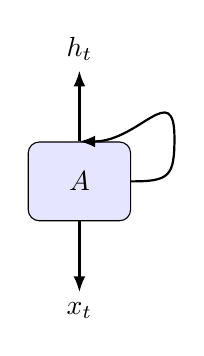
\begin{tikzpicture}[baseline]
  \node[draw, rounded corners, minimum width=1.3cm, minimum height=1cm, fill=blue!10] (A) {$A$};
  \draw[cline] (A.east) to [out=0,in=-90,looseness=1.6] ++(0.55,0.55) to [out=90,in=0,looseness=1.6] (A.north);
  \draw[cline] (A.south) -- ++(0,-0.9) node[below]{$x_t$};
  \draw[cline] (A.north) -- ++(0,0.9) node[above]{$h_t$};
\end{tikzpicture}
\caption{Dạng cuộn}
\end{subfigure}
\hfill
\begin{subfigure}[b]{0.74\textwidth}
\centering
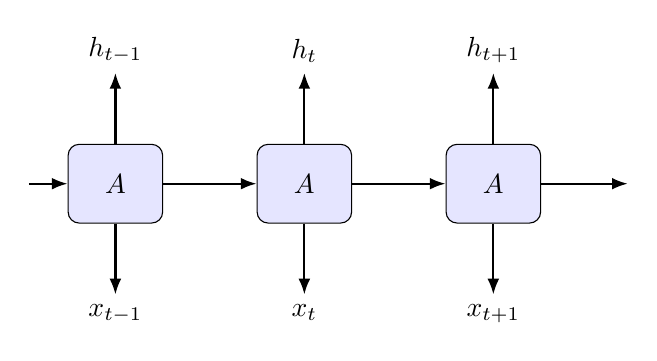
\begin{tikzpicture}[baseline]
  \node[draw, rounded corners, minimum width=1.2cm, minimum height=1cm, fill=blue!10] (A0) at (0,0) {$A$};
  \node[draw, rounded corners, minimum width=1.2cm, minimum height=1cm, fill=blue!10] (A1) at (2.4,0) {$A$};
  \node[draw, rounded corners, minimum width=1.2cm, minimum height=1cm, fill=blue!10] (A2) at (4.8,0) {$A$};
  \draw[cline] (A0.south) -- ++(0,-0.9) node[below]{$x_{t-1}$};
  \draw[cline] (A1.south) -- ++(0,-0.9) node[below]{$x_{t}$};
  \draw[cline] (A2.south) -- ++(0,-0.9) node[below]{$x_{t+1}$};
  \draw[cline] (A0.north) -- ++(0,0.9) node[above]{$h_{t-1}$};
  \draw[cline] (A1.north) -- ++(0,0.9) node[above]{$h_{t}$};
  \draw[cline] (A2.north) -- ++(0,0.9) node[above]{$h_{t+1}$};
  \draw[cline] (-1.1,0) -- (A0.west);
  \draw[cline] (A0.east) -- (A1.west);
  \draw[cline] (A1.east) -- (A2.west);
  \draw[cline] (A2.east) -- ++(1.1,0);
\end{tikzpicture}
\caption{Dạng khai triển theo thời gian (unrolled)}
\end{subfigure}
\caption{Kiến trúc Recurrent Neural Network (RNN)}
\label{fig:rnn}
\end{figure}

Hình~\ref{fig:rnn} minh họa một tế bào RNN $A$ ở hai cách biểu diễn: dạng cuộn (compact, với vòng lặp hồi quy) và dạng khai triển theo thời gian — trong đó cùng một tế bào $A$ (cùng bộ trọng số) được lặp lại tại mỗi bước, nhận đầu vào $x_t$ và trạng thái ẩn từ bước trước để tạo ra $h_t$.

\textbf{Vấn đề vanishing/exploding gradient.} Khi huấn luyện bằng lan truyền ngược qua thời gian (Backpropagation Through Time), đạo hàm của hàm mất mát theo các tham số ở những bước thời gian xa cần được tính thông qua tích của nhiều ma trận Jacobian — mỗi ma trận tương ứng với một bước thời gian:
\begin{equation}
\frac{\partial h_t}{\partial h_{t-k}} = \prod_{j=t-k+1}^{t} \frac{\partial h_j}{\partial h_{j-1}}
\end{equation}
Nếu các giá trị riêng (eigenvalue) của các ma trận Jacobian này liên tục nhỏ hơn 1, tích trên sẽ tiến dần về 0 khi $k$ tăng (\textbf{vanishing gradient}) — khiến mô hình gần như không học được các phụ thuộc xa; ngược lại nếu lớn hơn 1, tích sẽ bùng nổ (\textbf{exploding gradient}). Đây là hạn chế căn bản của RNN nguyên bản, làm động lực cho sự ra đời của LSTM.

\section{Long Short-Term Memory (LSTM)}

LSTM (Hochreiter và Schmidhuber, 1997) khắc phục vấn đề vanishing gradient của RNN bằng cách bổ sung một \textbf{trạng thái cell (cell state)} $C_t$ — một "đường cao tốc" thông tin chạy xuyên suốt chuỗi thời gian, chỉ trải qua các phép biến đổi tuyến tính đơn giản (nhân và cộng theo từng phần tử) thay vì phải đi qua hàm kích hoạt phi tuyến ở mỗi bước như trạng thái ẩn của RNN. Nhờ đó, gradient có thể lan truyền ngược qua nhiều bước thời gian mà ít bị suy giảm hơn.

LSTM điều khiển luồng thông tin ra/vào cell state thông qua ba \textbf{cổng (gate)}, mỗi cổng là một lớp sigmoid cho giá trị trong $[0,1]$ đóng vai trò "van" điều tiết:

\textbf{Cổng quên (Forget gate)} — quyết định giữ lại bao nhiêu phần trăm thông tin từ cell state cũ:
\begin{equation}
f_t = \sigma(W_f x_t + U_f h_{t-1} + b_f)
\end{equation}

\textbf{Cổng vào (Input gate)} và \textbf{trạng thái cell ứng viên} — quyết định thông tin mới nào sẽ được thêm vào:
\begin{equation}
i_t = \sigma(W_i x_t + U_i h_{t-1} + b_i)
\end{equation}
\begin{equation}
\tilde{C}_t = \tanh(W_C x_t + U_C h_{t-1} + b_C)
\end{equation}

\textbf{Cập nhật trạng thái cell} — kết hợp phần giữ lại (qua cổng quên) và phần thêm mới (qua cổng vào):
\begin{equation}
C_t = f_t \odot C_{t-1} + i_t \odot \tilde{C}_t
\end{equation}

\textbf{Cổng ra (Output gate)} và \textbf{trạng thái ẩn} — quyết định phần nào của cell state được "lộ ra" thành đầu ra:
\begin{equation}
o_t = \sigma(W_o x_t + U_o h_{t-1} + b_o)
\end{equation}
\begin{equation}
h_t = o_t \odot \tanh(C_t)
\end{equation}

\begin{figure}[H]
\centering
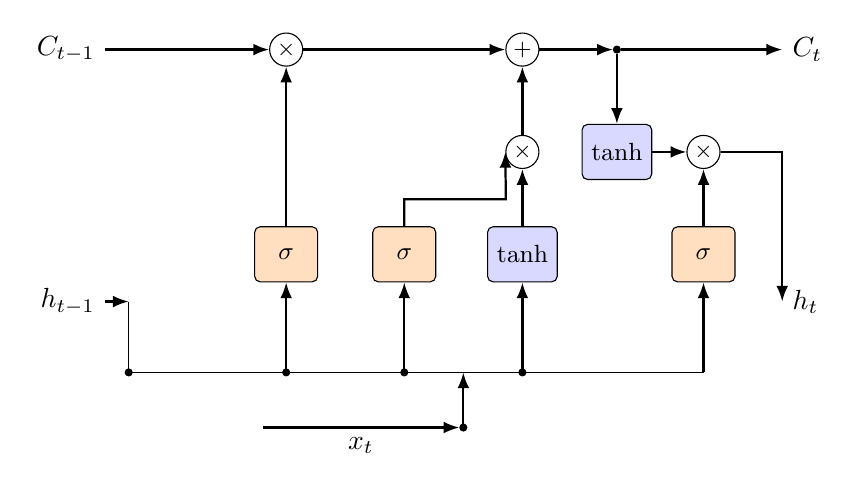
\begin{tikzpicture}[>=Latex]
  \node[opnode] (FM)  at (-4.5,3.2) {$\times$};
  \node[opnode] (ADD) at (-1.5,3.2) {$+$};
  \node[dotn]   (CT)  at (-0.3,3.2) {};

  \draw[cline] (-6.8,3.2) node[left]{$C_{t-1}$} -- (FM);
  \draw[cline] (FM) -- (ADD);
  \draw[cline] (ADD) -- (CT);
  \draw[cline] (CT) -- ++(2.1,0) node[right]{$C_t$};

  \node[opnode]  (IM)    at (-1.5,1.9) {$\times$};
  \node[tanhbox] (tanhC) at (-0.3,1.9) {$\tanh$};
  \node[opnode]  (OM)    at (0.8,1.9)  {$\times$};

  \draw[cline] (IM.north) -- (ADD.south);
  \draw[cline] (CT) -- (tanhC.north);
  \draw[cline] (tanhC.east) -- (OM.west);

  \node[gatebox] (f) at (-4.5,0.6) {$\sigma$};
  \node[gatebox] (i) at (-3.0,0.6) {$\sigma$};
  \node[tanhbox] (g) at (-1.5,0.6) {$\tanh$};
  \node[gatebox] (o) at (0.8,0.6)  {$\sigma$};

  \draw[cline] (f.north) -- (FM.south);
  \draw[cline] (g.north) -- (IM.south);
  \draw[cline] (i.north) -- (-3.0,1.3) -- (-1.71,1.3) -- (IM.west);
  \draw[cline] (o.north) -- (OM.south);

  \draw[cline] (-6.8,0.0) node[left]{$h_{t-1}$} -- (-6.5,0.0);
  \draw (-6.5,0.0) -- (-6.5,-0.9);
  \draw[cline] (OM.east) -- (1.8,1.9) -- (1.8,0.0) node[right]{$h_t$};

  \draw (-6.5,-0.9) -- (0.8,-0.9);
  \draw[cline] (-4.5,-0.9) -- (f.south);
  \draw[cline] (-3.0,-0.9) -- (i.south);
  \draw[cline] (-1.5,-0.9) -- (g.south);
  \draw[cline] (0.8,-0.9) -- (o.south);
  \node[dotn] at (-6.5,-0.9) {};
  \node[dotn] at (-4.5,-0.9) {};
  \node[dotn] at (-3.0,-0.9) {};
  \node[dotn] at (-1.5,-0.9) {};

  \node[dotn] (XD) at (-2.25,-1.6) {};
  \draw[cline] (XD) -- (-2.25,-0.9);
  \draw[cline] (-4.8,-1.6) -- (XD) node[midway,below]{$x_t$};
\end{tikzpicture}
\caption{Kiến trúc LSTM cell}
\label{fig:lstm}
\end{figure}

Hình~\ref{fig:lstm} minh họa luồng thông tin trong một tế bào LSTM: đường ngang phía trên (cell state $C_t$) chỉ tương tác với phần còn lại của mạng qua hai phép toán đơn giản (nhân với $f_t$, cộng với $i_t \odot \tilde{C}_t$); trạng thái ẩn $h_t$ được tính riêng ở đường phía dưới, là bản "lọc" của $\tanh(C_t)$ qua cổng ra $o_t$. Với ba cổng độc lập và một cell state riêng biệt, LSTM có nhiều tham số hơn RNN nhưng giải quyết hiệu quả vấn đề vanishing gradient, trở thành kiến trúc RNN có cổng được sử dụng rộng rãi nhất trong nhiều năm.

\section{Gated Recurrent Unit (GRU)}

GRU (Cho và cộng sự, 2014) là một biến thể \textbf{đơn giản hóa} của LSTM, được thiết kế với động lực giữ lại khả năng kiểm soát luồng thông tin dài hạn của LSTM nhưng với ít cổng và ít tham số hơn. So với LSTM, GRU có hai thay đổi cấu trúc chính:
\begin{itemize}
    \item \textbf{Gộp cổng quên và cổng vào} thành một \textbf{cổng cập nhật (update gate)} $z_t$ duy nhất, điều khiển đồng thời việc "quên" trạng thái cũ và "nạp" trạng thái mới thông qua một phép nội suy tuyến tính duy nhất.
    \item \textbf{Loại bỏ cell state riêng biệt}: GRU chỉ có một trạng thái ẩn $h_t$ duy nhất, vừa đóng vai trò "bộ nhớ dài hạn" (tương tự $C_t$ của LSTM) vừa là đầu ra tại mỗi bước — không cần cổng ra $o_t$ và phép biến đổi $\tanh(C_t)$ riêng như LSTM.
\end{itemize}

Tại mỗi bước thời gian $t$, với đầu vào $x_t$ và trạng thái ẩn trước đó $h_{t-1}$, GRU tính toán như sau:

\textbf{Cổng đặt lại (Reset gate)} — quyết định mức độ "quên" thông tin quá khứ khi tính trạng thái ứng viên:
\begin{equation}
r_t = \sigma(W_r x_t + U_r h_{t-1} + b_r)
\end{equation}

\textbf{Cổng cập nhật (Update gate)} — quyết định tỷ lệ giữa việc giữ lại trạng thái cũ và cập nhật bằng trạng thái ứng viên mới:
\begin{equation}
z_t = \sigma(W_z x_t + U_z h_{t-1} + b_z)
\end{equation}

\textbf{Trạng thái ẩn ứng viên (Candidate hidden state)}:
\begin{equation}
\tilde{h}_t = \tanh\big(W_h x_t + U_h (r_t \odot h_{t-1}) + b_h\big)
\end{equation}

\textbf{Trạng thái ẩn cập nhật} — nội suy tuyến tính giữa trạng thái cũ và trạng thái ứng viên, với hệ số nội suy do $z_t$ quyết định:
\begin{equation}
h_t = (1 - z_t) \odot h_{t-1} + z_t \odot \tilde{h}_t
\end{equation}

Trong đó $\sigma(\cdot)$ là hàm sigmoid, $\odot$ là phép nhân theo từng phần tử (Hadamard product), $W_{(\cdot)}, U_{(\cdot)}, b_{(\cdot)}$ là các trọng số và hệ số chệch cần học.

\begin{figure}[H]
\centering
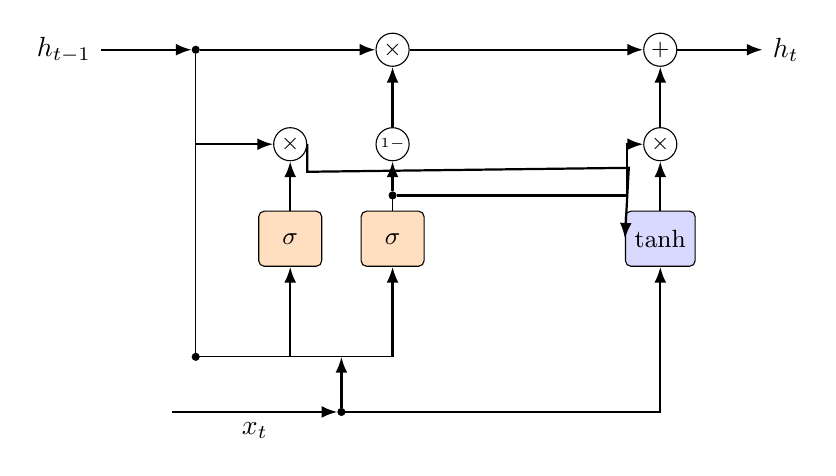
\begin{tikzpicture}[>=Latex]
  \node[dotn] (BD) at (-4.5,3.0) {};
  \node[opnode] (M1) at (-2.0,3.0) {$\times$};
  \node[opnode] (P)  at (1.4,3.0)  {$+$};

  \draw[cline] (-5.7,3.0) node[left]{$h_{t-1}$} -- (BD);
  \draw[cline] (BD) -- (M1);
  \draw[cline] (M1) -- (P);
  \draw[cline] (P) -- ++(1.3,0) node[right]{$h_t$};

  \node[opnode] (RM) at (-3.3,1.8) {$\times$};
  \node[opnode,font=\tiny] (ON) at (-2.0,1.8) {$1{-}$};
  \node[opnode] (M2) at (1.4,1.8)  {$\times$};

  \draw[cline] (ON.north) -- (M1.south);
  \draw (BD) -- (-4.5,1.8);
  \draw[cline] (-4.5,1.8) -- (RM.west);
  \draw[cline] (M2.north) -- (P.south);

  \node[gatebox] (r)  at (-3.3,0.6) {$\sigma$};
  \node[gatebox] (z)  at (-2.0,0.6) {$\sigma$};
  \node[tanhbox] (hc) at (1.4,0.6)  {$\tanh$};

  \draw[cline] (r.north) -- (RM.south);
  \node[dotn] (ZB) at (-2.0,1.15) {};
  \draw (z.north) -- (ZB);
  \draw[cline] (ZB) -- (ON.south);
  \draw[cline] (ZB) -- (0.98,1.15) -- (0.98,1.8) -- (M2.west);

  \draw[cline] (RM.east) -- ++(0,-0.35) -- (1.0,1.5) -- (hc.west);
  \draw[cline] (hc.north) -- (M2.south);

  \draw (BD) -- (-4.5,-0.9);
  \draw (-4.5,-0.9) -- (-2.0,-0.9);
  \draw[cline] (-3.3,-0.9) -- (r.south);
  \draw[cline] (-2.0,-0.9) -- (z.south);
  \node[dotn] at (-4.5,-0.9) {};

  \node[dotn] (XD) at (-2.65,-1.6) {};
  \draw[cline] (XD) -- (-2.65,-0.9);
  \draw[cline] (-4.8,-1.6) -- (XD) node[midway,below]{$x_t$};
  \draw[cline] (XD) -- (1.4,-1.6) -- (hc.south);
\end{tikzpicture}
\caption{Kiến trúc GRU cell}
\label{fig:gru}
\end{figure}

Hình~\ref{fig:gru} minh họa GRU: không còn đường cell state riêng như LSTM, trạng thái ẩn $h_{t-1}$ vừa đi thẳng vào phép nội suy $(1-z_t)\odot h_{t-1}$ (đường trên), vừa được điều tiết bởi cổng đặt lại $r_t$ trước khi tham gia tính trạng thái ứng viên $\tilde{h}_t$ (đường dưới). Khi $z_t \to 0$, trạng thái ẩn gần như được giữ nguyên qua bước thời gian — cơ chế then chốt giúp GRU giảm thiểu vanishing gradient tương tự cell state của LSTM; khi $z_t \to 1$, trạng thái được thay gần như hoàn toàn bằng trạng thái ứng viên mới.

Với bài toán dự báo hồi quy (không phải phân loại) tại một horizon $h$ cố định, cho trước ($h \geq 1$ là số bước thời gian cần dự báo trước, được chọn trước khi huấn luyện), đầu ra cuối cùng của mô hình là trạng thái ẩn tại bước thời gian cuối của cửa sổ đầu vào, đưa qua một lớp fully-connected tuyến tính để cho ra giá trị dự báo của biến mục tiêu tại bước $t+h$:
\begin{equation}
\hat{y}_{t+h} = W_{fc}\, h_{w} + b_{fc}
\end{equation}
với $h_w$ là trạng thái ẩn tại bước cuối cùng ($w$) của cửa sổ đầu vào. Horizon $h$ ở đây là một \textbf{siêu tham số kiến trúc}: mỗi model chỉ được huấn luyện để dự báo đúng một giá trị $h$ duy nhất — muốn đổi sang horizon khác phải huấn luyện lại từ đầu.

Trong thực tế, nhiều bài toán cần dự báo \textbf{đồng thời nhiều horizon khác nhau} (chẳng hạn cả $1, 2, \dots, H$ bước tới cùng lúc), thay vì chỉ một $h$ duy nhất như kiến trúc cơ sở ở trên. Hai chiến lược phổ biến để mở rộng một model một-horizon sang dự báo $H$ bước tương lai được trình bày dưới đây.

\subsection*{Recursive GRU}

Cách đơn giản nhất để dự báo nhiều bước mà \textbf{không cần huấn luyện lại} là tái sử dụng nguyên một model đã huấn luyện sẵn cho horizon $h=1$ (kiến trúc ở trên với $h=1$) — bắt buộc phải là $h=1$ vì đây là đơn vị bước nhỏ nhất, mỗi lần gọi model chỉ trượt cửa sổ đi đúng 1 bước, nhờ đó có thể gọi lặp lại $H$ lần liên tiếp để đi xa dần — gọi là chiến lược \textbf{Recursive (đệ quy)}.

Tại bước thứ $k$ ($k = 1, \dots, H$), model nhận cửa sổ $w$ giờ gần nhất và cho ra dự đoán:
\begin{equation}
\hat{y}_{t+k} = f_\theta\big(\tilde{x}_{t-w+k}, \dots, \tilde{x}_{t-1+k}\big)
\end{equation}
trong đó $f_\theta$ là model GRU horizon=1 đã huấn luyện, và $\tilde{x}_i$ là vector đặc trưng "tổng hợp" tại thời điểm $i$: nếu $i \leq t$ (đã có dữ liệu thật) thì $\tilde{x}_i = x_i$; nếu $i > t$ (thuộc tương lai, chưa quan trắc) thì thành phần mục tiêu (biến cần dự báo) của $\tilde{x}_i$ được thay bằng chính giá trị model \textbf{vừa dự đoán} ở bước trước đó ($\hat{y}_i$), còn các thành phần đặc trưng ngoại sinh khác thường dùng \textbf{persistence} — giữ nguyên giá trị thật cuối cùng đã biết, do chưa có dự báo riêng cho chúng — trừ những đặc trưng có thể tính \textbf{chính xác} cho tương lai (ví dụ đặc trưng thời gian dạng chu kỳ, vốn là hàm xác định, không cần dự báo).

\begin{figure}[H]
\centering
\begin{tikzpicture}[>=Latex, x=1cm, y=1cm]
  \node[realcell] at (0,4.3) {};
  \node[right, font=\scriptsize] at (0.5,4.3) {Dữ liệu thật};
  \node[predcell] at (3.2,4.3) {};
  \node[right, font=\scriptsize] at (3.7,4.3) {Model tự dự đoán};

  \node[font=\small\bfseries] at (-2.3,3) {Bước 1};
  \foreach \i in {0,1,2,3} {
    \node[realcell] (a\i) at (\i*0.9,3) {};
  }
  \node[grubox] (g1) at (4.6,3) {GRU};
  \draw[cline] (a3.east) -- (g1.west);
  \draw[cline] (g1.east) -- ++(0.9,0) node[predcell,right=0.05cm,font=\scriptsize] (p1) {$\hat y_{w+1}$};

  \node[font=\small\bfseries] at (-2.3,1.6) {Bước 2};
  \foreach \i in {0,1,2} {
    \node[realcell] (b\i) at (\i*0.9,1.6) {};
  }
  \node[predcell] (b3) at (2.7,1.6) {$\hat y_{w+1}$};
  \node[grubox] (g2) at (4.6,1.6) {GRU};
  \draw[cline] (b3.east) -- (g2.west);
  \draw[cline] (g2.east) -- ++(0.9,0) node[predcell,right=0.05cm,font=\scriptsize] (p2) {$\hat y_{w+2}$};

  \node[font=\small\bfseries] at (-2.3,0.2) {Bước 3};
  \node[realcell] (c0) at (0,0.2) {};
  \node[realcell] (c1) at (0.9,0.2) {};
  \node[predcell] (c2) at (1.8,0.2) {$\hat y_{w+1}$};
  \node[predcell] (c3) at (2.7,0.2) {$\hat y_{w+2}$};
  \node[grubox] (g3) at (4.6,0.2) {GRU};
  \draw[cline] (c3.east) -- (g3.west);
  \draw[cline] (g3.east) -- ++(0.9,0) node[predcell,right=0.05cm,font=\scriptsize] (p3) {$\hat y_{w+3}$};

  \draw[-{Latex[length=1.5mm]}, gray, dashed] (p1.south) to[out=-90,in=90] (b3.north);
  \draw[-{Latex[length=1.5mm]}, gray, dashed] (p2.south) to[out=-90,in=90] (c3.north);
\end{tikzpicture}
\caption{Recursive GRU: cửa sổ trượt, phần dự đoán ở bước trước bị đưa ngược vào làm input cho bước sau}
\label{fig:recursive}
\end{figure}

Hình~\ref{fig:recursive} minh họa cơ chế này qua 3 bước đầu tiên: ở Bước 1, cửa sổ input hoàn toàn là dữ liệu thật; sang Bước 2, giá trị $\hat{y}_{w+1}$ vừa sinh ra ở Bước 1 được "trượt" vào cửa sổ, thay thế cho phần dữ liệu thật cũ nhất bị loại ra; đến Bước 3, cửa sổ đã chứa 2 giá trị tự dự đoán. Càng dự đoán xa, tỷ lệ dữ liệu thật trong cửa sổ càng giảm, dần được thay thế bởi chính dự đoán của model.

\textbf{Ưu điểm}: không cần huấn luyện model mới, tận dụng nguyên vẹn model horizon=1 đã có sẵn.

\textbf{Nhược điểm}: vì $\hat{y}_{t+k}$ phụ thuộc vào các dự đoán $\hat{y}_{t+1}, \dots, \hat{y}_{t+k-1}$ ở những bước trước (thay vì dữ liệu thật), sai số của mỗi bước sẽ \textbf{dồn tích} (error compounding) qua các bước tiếp theo — bước dự đoán càng xa mốc gốc, độ tin cậy càng giảm nhanh. Ngoài ra, giả định persistence cho các đặc trưng ngoại sinh cũng là một nguồn sai lệch bổ sung nếu các đặc trưng này thực sự biến động trong giai đoạn dự báo.

\subsection*{Direct GRU (Vector Output)}

Chiến lược thứ hai giải quyết trực tiếp vấn đề dồn sai số của Recursive: thay vì tái sử dụng model horizon=1, \textbf{huấn luyện một model mới} dự đoán \textbf{toàn bộ $H$ bước tương lai cùng lúc} trong một lần forward pass duy nhất.

Kiến trúc Encoder GRU được giữ nguyên như đã trình bày ở trên (đọc cửa sổ $w$ giờ lịch sử, nén thành trạng thái ẩn cuối $h_w$), chỉ thay đổi duy nhất lớp fully-connected: thay vì $\text{Linear}(\text{hidden}, 1)$ chỉ ra một số, dùng $\text{Linear}(\text{hidden}, H)$ để ra thẳng $H$ giá trị cùng lúc:
\begin{equation}
[\hat{y}_{t+1}, \hat{y}_{t+2}, \dots, \hat{y}_{t+H}]^\top = W_{fc}\, h_w + b_{fc}, \qquad W_{fc} \in \mathbb{R}^{H \times \text{hidden}}
\end{equation}

\begin{figure}[H]
\centering
\begin{tikzpicture}[>=Latex, x=1cm, y=1cm]
  \foreach \i in {0,1,2,3} {
    \node[realcell] (a\i) at (\i*0.9,0) {};
  }
  \node[font=\scriptsize] at (1.35,-0.6) {Cửa sổ input (toàn bộ dữ liệu thật)};

  \node[grubox, minimum width=1.6cm, minimum height=1cm] (enc) at (5.2,0) {Encoder GRU};
  \draw[cline] (a3.east) -- (enc.west);

  \node[opnode, minimum size=0.5cm] (hw) at (7.3,0) {$h_w$};
  \draw[cline] (enc.east) -- (hw.west);

  \node[gatebox, fill=violet!15, minimum width=1.4cm] (fc) at (9.4,0) {Linear};
  \draw[cline] (hw.east) -- (fc.west);

  \node[predcell] (o1) at (11.6,1.65) {$\hat y_{w+1}$};
  \node[predcell] (o2) at (11.6,0.55) {$\hat y_{w+2}$};
  \node[font=\small] (odots) at (11.6,-0.55) {$\vdots$};
  \node[predcell] (oH) at (11.6,-1.65) {$\hat y_{w+H}$};
  \foreach \o in {o1,o2,oH} {
    \draw[cline] (fc.east) -- (\o.west);
  }

  \node[font=\scriptsize] at (9.4,-2.6) {1 lần forward pass duy nhất};
\end{tikzpicture}
\caption{Direct GRU: một Encoder duy nhất, output rộng ra thẳng cả $H$ bước cùng lúc, không đệ quy}
\label{fig:direct}
\end{figure}

Hình~\ref{fig:direct} cho thấy điểm khác biệt cốt lõi so với Recursive: cửa sổ input \textbf{luôn là dữ liệu thật 100\%} — không có bước dự đoán nào bị đưa ngược lại làm input cho bước khác. Toàn bộ $H$ dự đoán đều được tính \textbf{độc lập với nhau}, xuất phát từ cùng một ngữ cảnh $h_w$ duy nhất.

\textbf{Ưu điểm}: vì không có cơ chế đệ quy, Direct GRU \textbf{không bị dồn sai số} qua các bước horizon — sai số ở bước dự đoán xa không phụ thuộc vào sai số ở bước gần.

\textbf{Nhược điểm}: model phải học đồng thời $H$ mục tiêu khác nhau trong cùng một mạng (đa nhiệm), có thể đánh đổi đôi chút độ chính xác ở bước dự đoán gần nhất ($h=1$) so với một model được huấn luyện chuyên biệt chỉ cho horizon=1 duy nhất; đồng thời cần huấn luyện lại từ đầu, không tái sử dụng được model horizon=1 sẵn có như Recursive.

% ==================== CHƯƠNG 2: ỨNG DỤNG ====================
\chapter{Ứng dụng}

\section{Mô tả dữ liệu}

Bộ dữ liệu gốc (\texttt{raw\_data.csv}) được tải trực tiếp từ Open-Meteo Air Quality API, trải dài từ năm 2016 nhưng phần lớn giai đoạn đầu (2016 -- giữa 2022) không có dữ liệu (toàn bộ giá trị NaN) do trạm quan trắc/API chưa cung cấp dữ liệu ở giai đoạn đó. Sau bước làm sạch (loại bỏ các hàng toàn NaN và các cột chứa NaN — trong đó \texttt{carbon\_dioxide} và \texttt{methane} bị loại hoàn toàn vì chỉ có dữ liệu một phần thời gian), bộ dữ liệu sạch (\texttt{cleaned\_data.csv}) còn lại \textbf{34.865 dòng $\times$ 15 cột}, liên tục theo từng giờ từ \texttt{2022-08-04 07:00:00} đến \texttt{2026-07-26 23:00:00}, không còn giá trị thiếu.

Các biến trong bộ dữ liệu sau khi chuẩn hóa tên cột:

\begin{itemize}
    \item \textbf{PM10}: Nồng độ bụi mịn đường kính $\leq 10\,\mu$m ($\mu$g/m$^3$)
    \item \textbf{PM2.5}: Nồng độ bụi mịn đường kính $\leq 2.5\,\mu$m ($\mu$g/m$^3$) — \textit{biến mục tiêu}
    \item \textbf{Carbon Monoxide (CO)}: Khí carbon monoxide ($\mu$g/m$^3$)
    \item \textbf{Nitrogen Dioxide (NO$_2$)}: Khí nitơ đioxit ($\mu$g/m$^3$)
    \item \textbf{Sulphur Dioxide (SO$_2$)}: Khí lưu huỳnh đioxit ($\mu$g/m$^3$)
    \item \textbf{Ozone (O$_3$)}: Khí ozone tầng mặt đất ($\mu$g/m$^3$)
    \item \textbf{Aerosol Optical Depth (AOD)}: Độ dày quang học sol khí, phản ánh mức độ khí quyển bị che khuất bởi hạt lơ lửng (không đơn vị)
    \item \textbf{Dust}: Nồng độ bụi ($\mu$g/m$^3$)
    \item \textbf{UV Index}, \textbf{UV Index Clear Sky}: Chỉ số tia UV thực tế và giả định trời quang mây (không đơn vị)
    \item \textbf{day, month, year, hour}: Các thành phần thời gian tách từ cột \texttt{time}
\end{itemize}

\begin{table}[H]
\centering
\caption{Thống kê mô tả các biến định lượng}
\label{tab:describe}
\begin{tabular}{lrrrrrr}
\toprule
Biến & Đơn vị & Mean & Std & Min & Median & Max \\
\midrule
PM10 & $\mu$g/m$^3$ & 19.76 & 9.91 & 0.40 & 18.20 & 97.80 \\
PM2.5 & $\mu$g/m$^3$ & 13.73 & 7.06 & 0.30 & 12.50 & 71.50 \\
Carbon Monoxide & $\mu$g/m$^3$ & 249.38 & 109.28 & 59.00 & 226.00 & 1185.00 \\
Nitrogen Dioxide & $\mu$g/m$^3$ & 3.05 & 2.59 & 0.00 & 2.30 & 29.30 \\
Sulphur Dioxide & $\mu$g/m$^3$ & 2.23 & 1.37 & 0.10 & 1.90 & 13.50 \\
Ozone & $\mu$g/m$^3$ & 81.58 & 30.30 & 4.00 & 79.00 & 259.00 \\
Aerosol Optical Depth & --- & 0.25 & 0.16 & 0.02 & 0.21 & 2.37 \\
Dust & $\mu$g/m$^3$ & 0.42 & 1.45 & 0.00 & 0.00 & 37.00 \\
UV Index & --- & 2.01 & 3.21 & 0.00 & 0.00 & 13.65 \\
UV Index Clear Sky & --- & 2.53 & 3.84 & 0.00 & 0.00 & 14.10 \\
\bottomrule
\end{tabular}
\end{table}

Ba biến cuối (\textit{Dust}, \textit{UV Index}, \textit{UV Index Clear Sky}) có trung vị bằng 0, cho thấy phân phối lệch phải rất mạnh với phần lớn giá trị bằng 0 — dấu hiệu cho thấy các biến này có thể ít mang thông tin hữu ích cho việc dự báo PM2.5, sẽ được kiểm chứng qua phân tích tương quan ở phần tiếp theo.

\section{Phân tích khám phá dữ liệu (EDA)}

\subsection*{Tương quan giữa các chỉ số chất lượng không khí}

\begin{figure}[H]
\centering
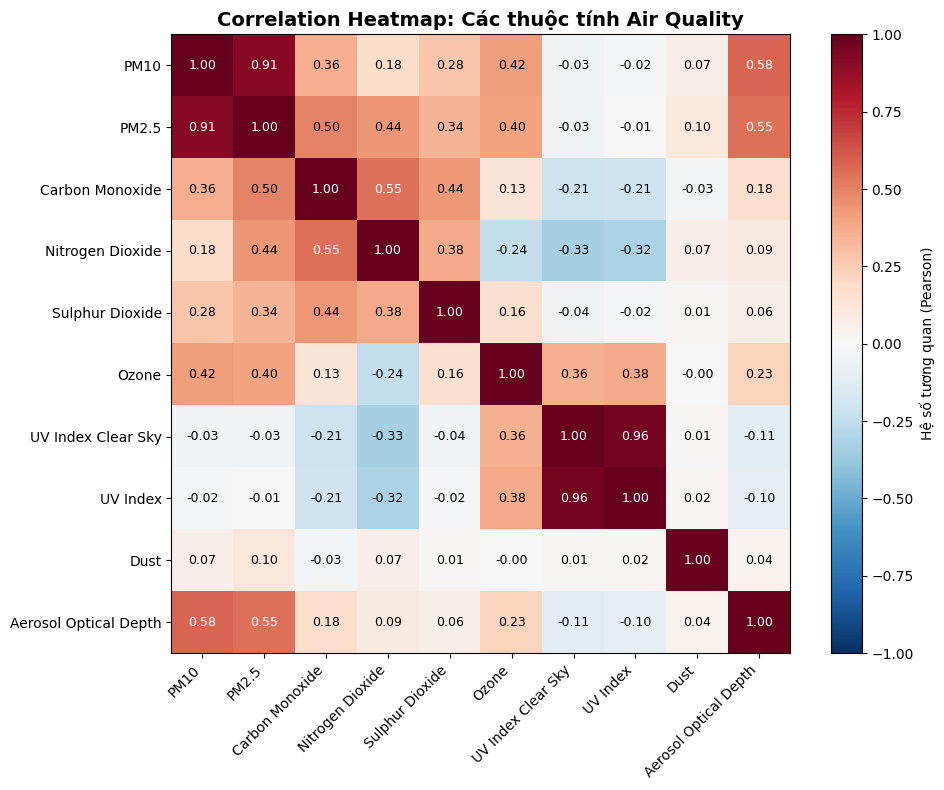
\includegraphics[width=0.75\textwidth]{figures/correlation_heatmap.png}
\caption{Ma trận tương quan Pearson giữa các chỉ số chất lượng không khí}
\label{fig:corr}
\end{figure}

Hình~\ref{fig:corr} cho thấy PM10 và PM2.5 có tương quan rất cao ($r = 0.91$) — phù hợp với thực tế vì PM2.5 là tập con của PM10. PM2.5 cũng có tương quan trung bình với Carbon Monoxide ($r=0.50$), Nitrogen Dioxide ($r=0.44$) và Aerosol Optical Depth ($r=0.55$) — các chỉ số phần lớn liên quan đến hoạt động đốt cháy (giao thông, công nghiệp). Ngược lại, Dust ($r=0.10$) và UV Index/UV Index Clear Sky ($r \approx -0.01$ đến $-0.03$) gần như không tương quan với PM2.5 — nhất quán với nhận xét về phân phối lệch ở trên.

\subsection*{Xu hướng và phân phối theo thời gian}

\begin{figure}[H]
\centering
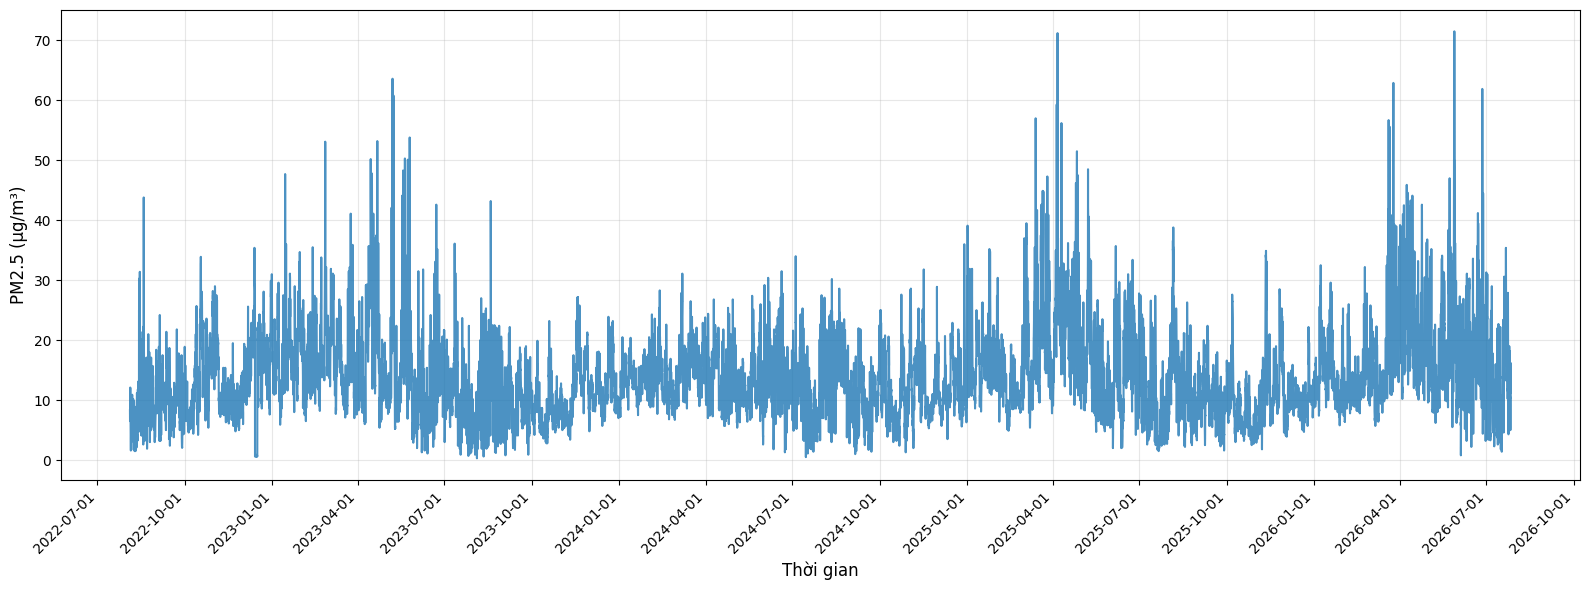
\includegraphics[width=\textwidth]{figures/pm25_lineplot.png}
\caption{Chuỗi thời gian nồng độ PM2.5 (2022--2026)}
\label{fig:lineplot}
\end{figure}

\begin{figure}[H]
\centering
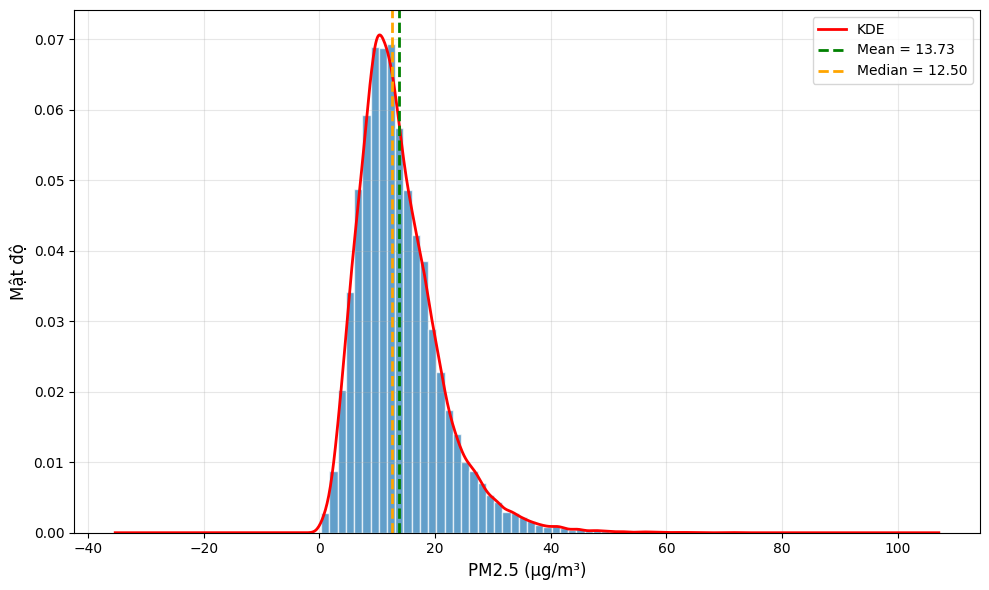
\includegraphics[width=0.7\textwidth]{figures/pm25_histogram.png}
\caption{Phân phối PM2.5: Histogram và ước lượng mật độ (KDE)}
\label{fig:hist}
\end{figure}

Chuỗi PM2.5 (Hình~\ref{fig:lineplot}) dao động chủ yếu trong khoảng 5--30~$\mu$g/m$^3$, với các đợt tăng đột biến ngắn hạn (lên đến $\sim$70~$\mu$g/m$^3$) và biểu hiện lặp lại theo mùa khá rõ. Phân phối PM2.5 (Hình~\ref{fig:hist}) lệch phải, với giá trị trung vị (12.5) thấp hơn giá trị trung bình (13.73) — phù hợp với đặc điểm dữ liệu môi trường, nơi các sự kiện ô nhiễm cao là thiểu số nhưng có biên độ lớn.

\subsection*{Tính dừng và xu hướng dài hạn}

Để xác định chuỗi PM2.5 có xu hướng dài hạn hay không — yếu tố quan trọng khi lựa chọn cách biểu diễn đầu vào cho mô hình — hai kiểm định tính dừng (ADF và KPSS) và kiểm định xu hướng phi tham số Mann-Kendall được áp dụng trên chuỗi PM2.5 trung bình ngày.

\begin{table}[H]
\centering
\caption{Kết quả kiểm định tính dừng (PM2.5 trung bình ngày)}
\begin{tabular}{lrrl}
\toprule
Kiểm định & Thống kê & p-value & Kết luận \\
\midrule
ADF (H0: có unit root) & $-5.999$ & $<0.0001$ & Dừng (bác bỏ H0) \\
KPSS (H0: dừng) & $0.277$ & $0.10$ & Dừng (không bác bỏ H0) \\
\bottomrule
\end{tabular}
\end{table}

Cả hai kiểm định đều đồng thuận: chuỗi PM2.5 là \textbf{chuỗi dừng} (stationary) — không tồn tại xu hướng ngẫu nhiên (stochastic trend) dài hạn. Kết quả này được củng cố thêm bởi kiểm định \textbf{Seasonal Mann-Kendall} trên PM2.5 trung bình tháng: xu hướng ước lượng là \textit{"no trend"} với $p = 0.7686$ (không đủ bằng chứng thống kê để bác bỏ giả thuyết không có xu hướng đơn điệu), độ dốc Sen's slope chỉ $0.28\,\mu$g/m$^3$/tháng ($\approx 3.3\,\mu$g/m$^3$/năm) — rất nhỏ so với độ lệch chuẩn của chuỗi ($7.06\,\mu$g/m$^3$). Nói cách khác, biến động của PM2.5 trong giai đoạn quan sát chủ yếu đến từ \textbf{tính chu kỳ (seasonality)} chứ không phải từ một xu hướng tăng/giảm dài hạn rõ rệt.

\subsection*{Tính chu kỳ (Seasonality)}

\begin{figure}[H]
\centering
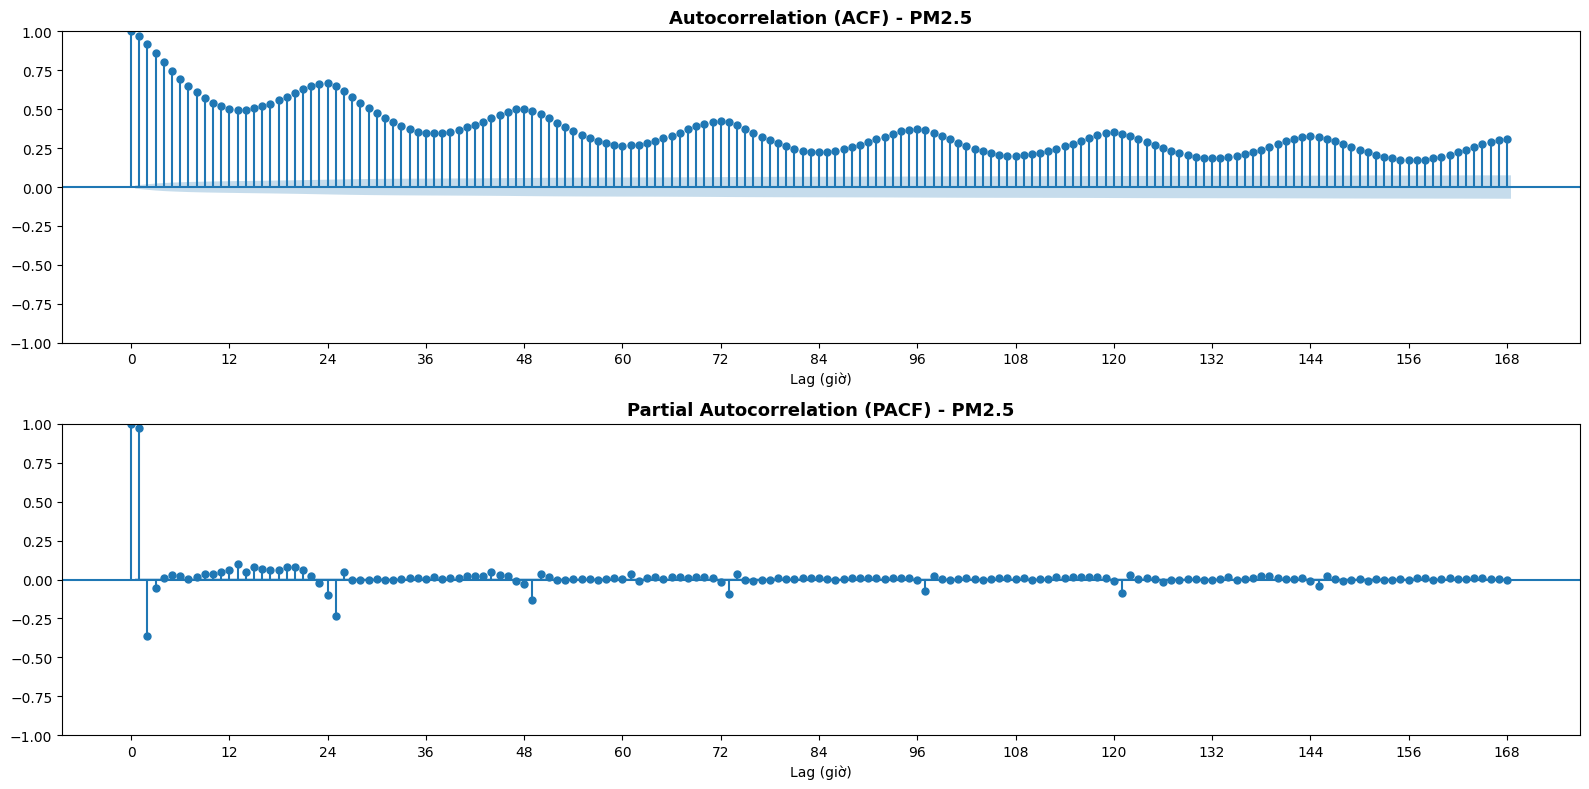
\includegraphics[width=\textwidth]{figures/acf_pacf.png}
\caption{ACF và PACF của PM2.5 theo giờ (168 lag $=$ 1 tuần)}
\label{fig:acfpacf}
\end{figure}

Biểu đồ ACF (Hình~\ref{fig:acfpacf}) thể hiện các đỉnh lặp lại rõ rệt tại lag 24, 48, 72, 96... giờ — xác nhận \textbf{chu kỳ ngày (24 giờ)} là chu kỳ chi phối hành vi ngắn hạn của PM2.5, phù hợp với quy luật sinh hoạt/giao thông đô thị (giờ cao điểm) lặp lại mỗi ngày. Đây là căn cứ quan trọng để lựa chọn kích thước cửa sổ đầu vào (window size) cho mô hình ở Mục~2.4.

\begin{figure}[H]
\centering
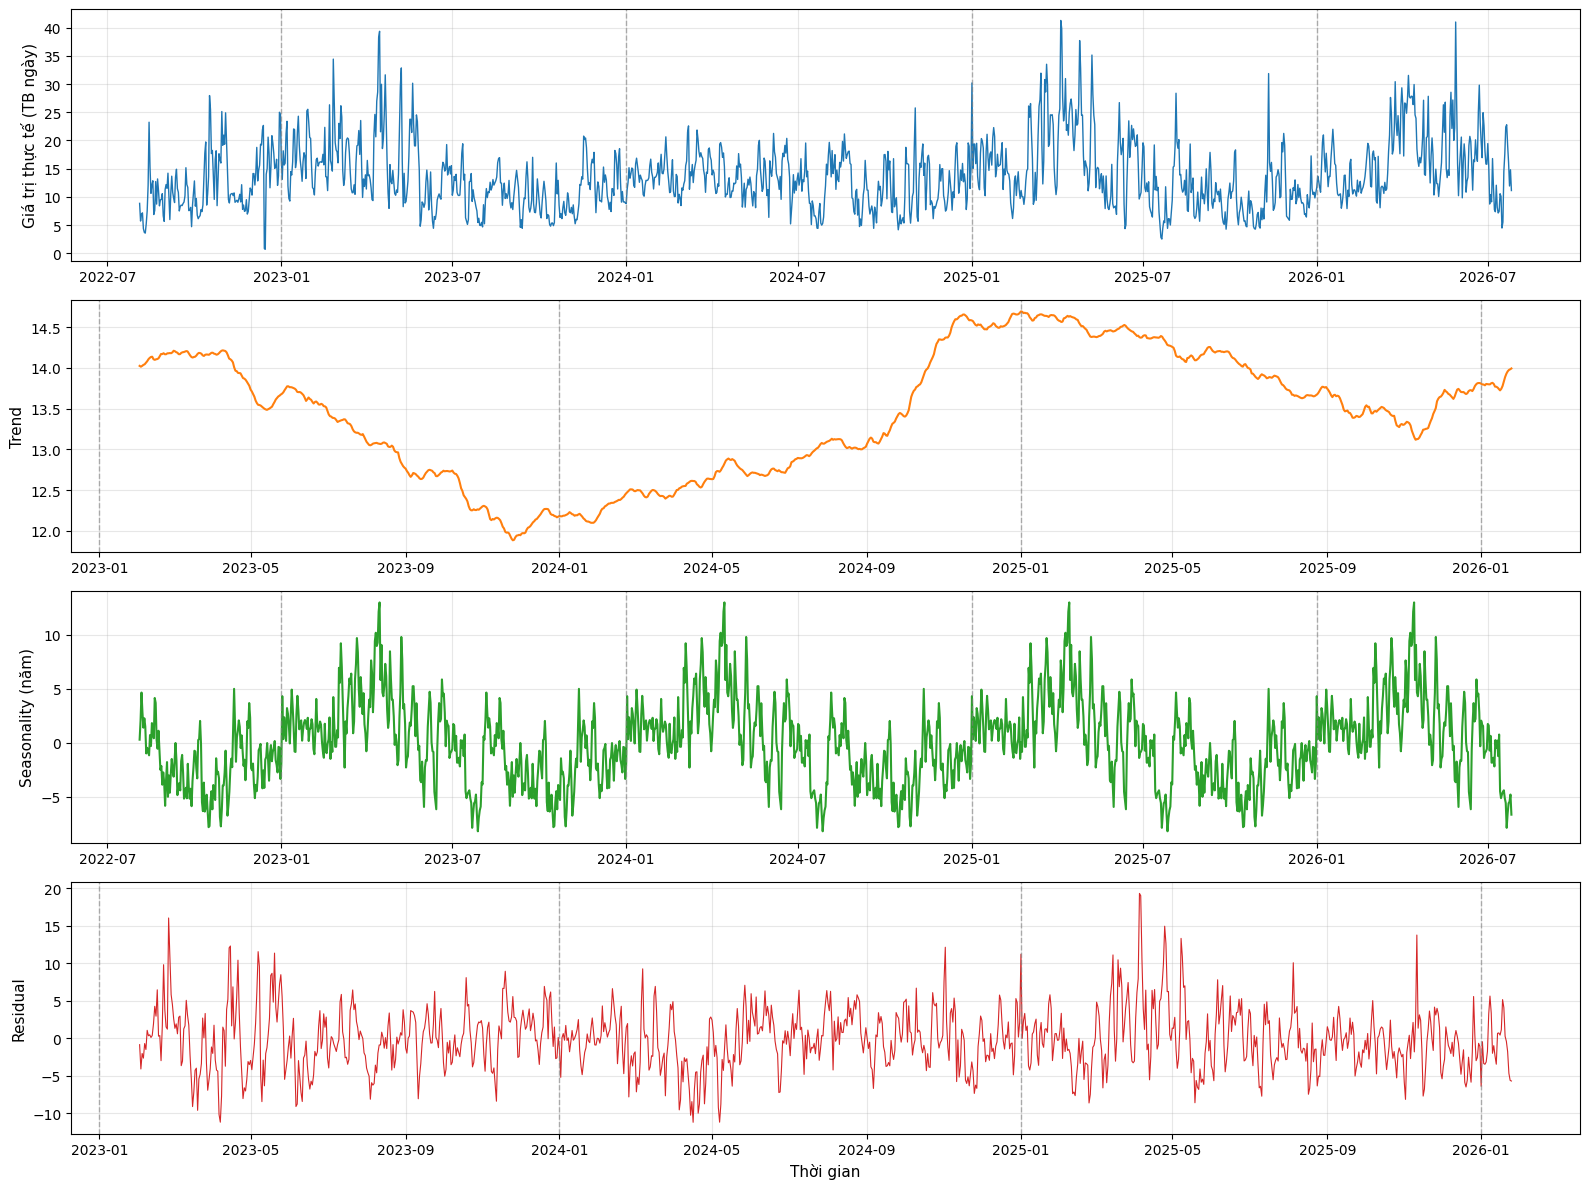
\includegraphics[width=\textwidth]{figures/decomposition.png}
\caption{Phân rã chuỗi thời gian PM2.5 theo chu kỳ năm (Trend + Seasonal + Residual)}
\label{fig:decomp}
\end{figure}

Phân rã cổ điển (Hình~\ref{fig:decomp}, period$=365$ ngày trên chuỗi trung bình ngày) cho thấy thành phần Trend dao động nhẹ trong khoảng 12--14.7, không có xu hướng đơn điệu rõ ràng — nhất quán với kết luận từ Mann-Kendall. Thành phần Residual sau phân rã được kiểm định Ljung-Box tại các lag 10, 20, 30, 60, 90: kết quả cho thấy vẫn còn tự tương quan có ý nghĩa thống kê ở một số lag, nghĩa là phân rã cổ điển theo chu kỳ năm chưa tách hết toàn bộ cấu trúc chuỗi — phù hợp với thực tế vì chuỗi còn chứa chu kỳ ngày (24h) mà phép phân rã theo period$=365$ không nắm bắt được.

\begin{figure}[H]
\centering
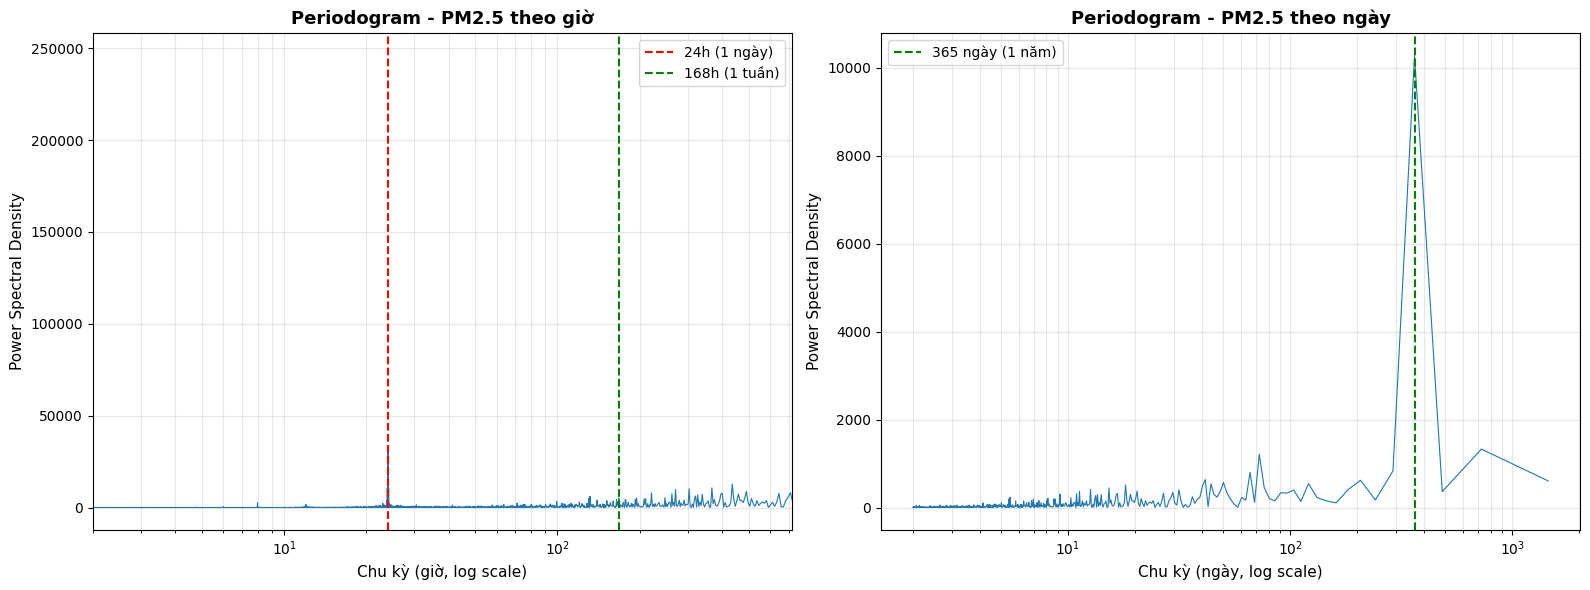
\includegraphics[width=\textwidth]{figures/periodogram.png}
\caption{Periodogram (FFT) của PM2.5 — xác nhận các chu kỳ chiếm ưu thế}
\label{fig:periodogram}
\end{figure}

Phân tích phổ tần số bằng Periodogram (Hình~\ref{fig:periodogram}) — không giả định trước chu kỳ mà quét toàn bộ phổ — xác nhận hai chu kỳ chiếm ưu thế: chu kỳ \textbf{năm ($\approx$363 ngày, power $\approx$246.036)} là mạnh nhất, tiếp theo là chu kỳ \textbf{ngày (24h, power $\approx$31.241)}. Các đỉnh phụ tại 72.6, 41.5 ngày... đều là ước số của $\approx$365 nên là các họa ba (harmonics) của chu kỳ năm, không phải chu kỳ độc lập mới. Điều này cho thấy PM2.5 tại Quy Nhơn chịu ảnh hưởng rõ rệt bởi cả biến động mùa trong năm (gió mùa, thời tiết) lẫn nhịp sinh hoạt hàng ngày.

\subsection*{Xu hướng theo Moving Average}

\begin{figure}[H]
\centering
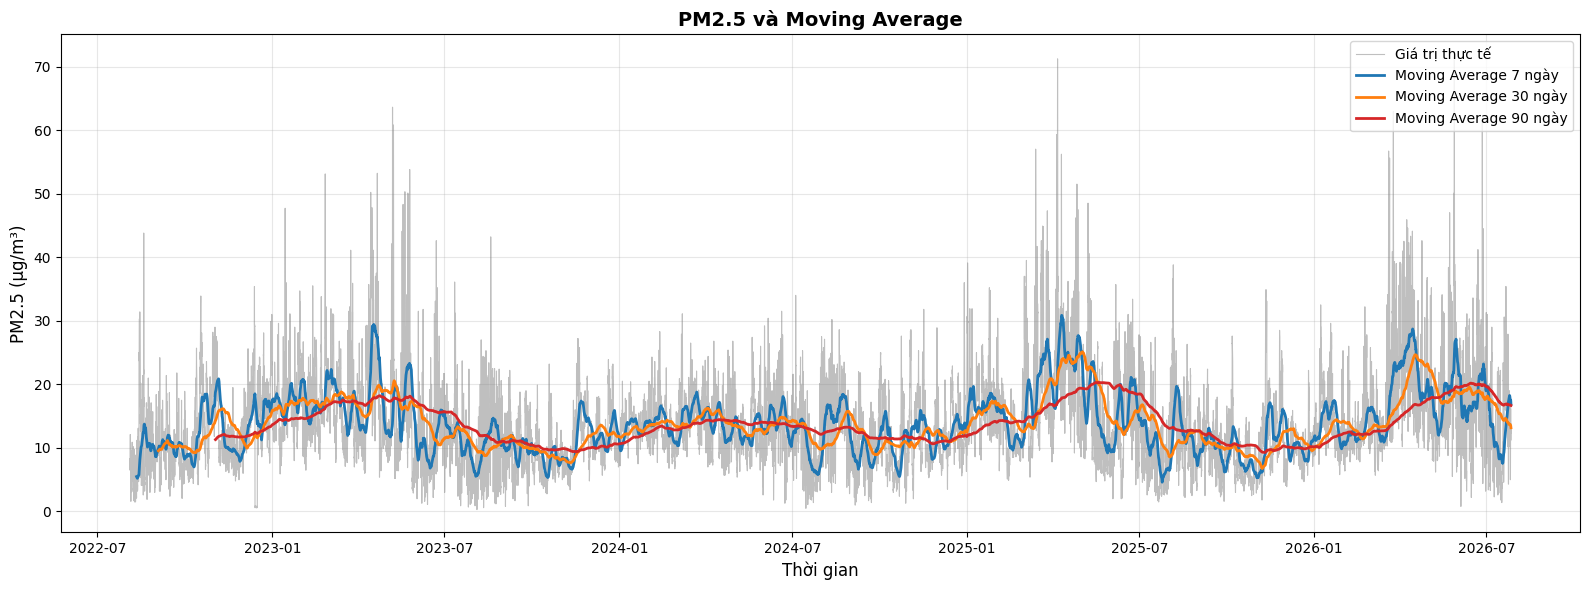
\includegraphics[width=\textwidth]{figures/pm25_moving_average.png}
\caption{PM2.5 và đường trung bình trượt (Moving Average) 7, 30 và 90 ngày}
\label{fig:ma}
\end{figure}

Hình~\ref{fig:ma} cho thấy các đường trung bình trượt 30 ngày và 90 ngày dao động lặp lại theo chu kỳ hàng năm — tăng vào giai đoạn đầu năm (khoảng tháng 1--4) và giảm dần về giữa năm — chứ không trôi dạt theo một hướng cố định qua các năm 2022--2026, nhất quán với kết luận "không có xu hướng đơn điệu" từ kiểm định Mann-Kendall đã trình bày ở trên. Chuỗi giá trị thực tế (đường xám) dao động rất mạnh quanh các đường trung bình trượt, phản ánh nhiều đợt tăng đột biến ngắn hạn xen kẽ nền chu kỳ mùa.

\subsection*{Phân phối PM2.5 theo từng năm}

\begin{figure}[H]
\centering
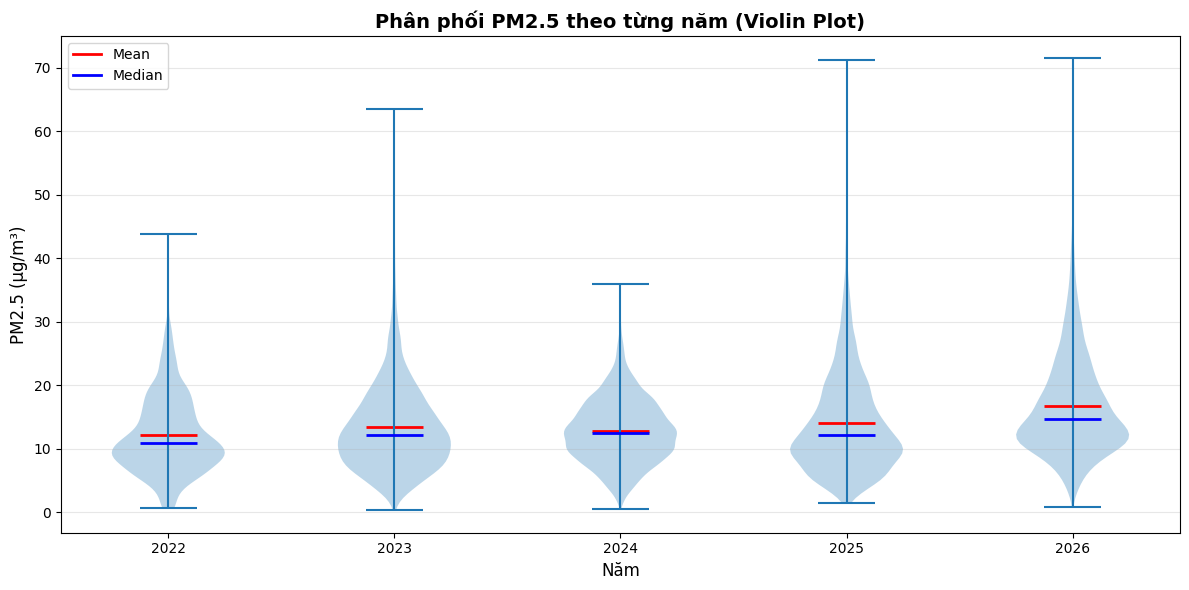
\includegraphics[width=0.85\textwidth]{figures/pm25_violin_year.png}
\caption{Phân phối PM2.5 theo từng năm (Violin Plot)}
\label{fig:violin}
\end{figure}

Hình~\ref{fig:violin} cho thấy giá trị trung vị/trung bình PM2.5 tương đối ổn định quanh 11--14~$\mu$g/m$^3$ trong giai đoạn 2022--2025, nhưng giá trị cực đại (đuôi phân phối) có xu hướng tăng dần qua từng năm — từ khoảng 44~$\mu$g/m$^3$ (2022) lên hơn 70~$\mu$g/m$^3$ (2025--2026) — cho thấy dù mức nền không đổi nhiều nhưng tần suất/cường độ các đợt ô nhiễm đỉnh điểm có dấu hiệu gia tăng. Riêng năm 2026 (dữ liệu mới tính đến tháng 7) có phân phối lệch cao hơn hẳn (trung vị $\approx$14.5) so với các năm trước; tuy nhiên cần lưu ý đây là năm chưa có đủ dữ liệu cả năm, nên tỷ trọng các tháng đầu năm — vốn có PM2.5 cao hơn theo Hình~\ref{fig:seasonal} — chiếm phần lớn có thể ảnh hưởng đến so sánh này.

\subsection*{Ngưỡng an toàn theo chuẩn WHO và QCVN Việt Nam}

\begin{figure}[H]
\centering
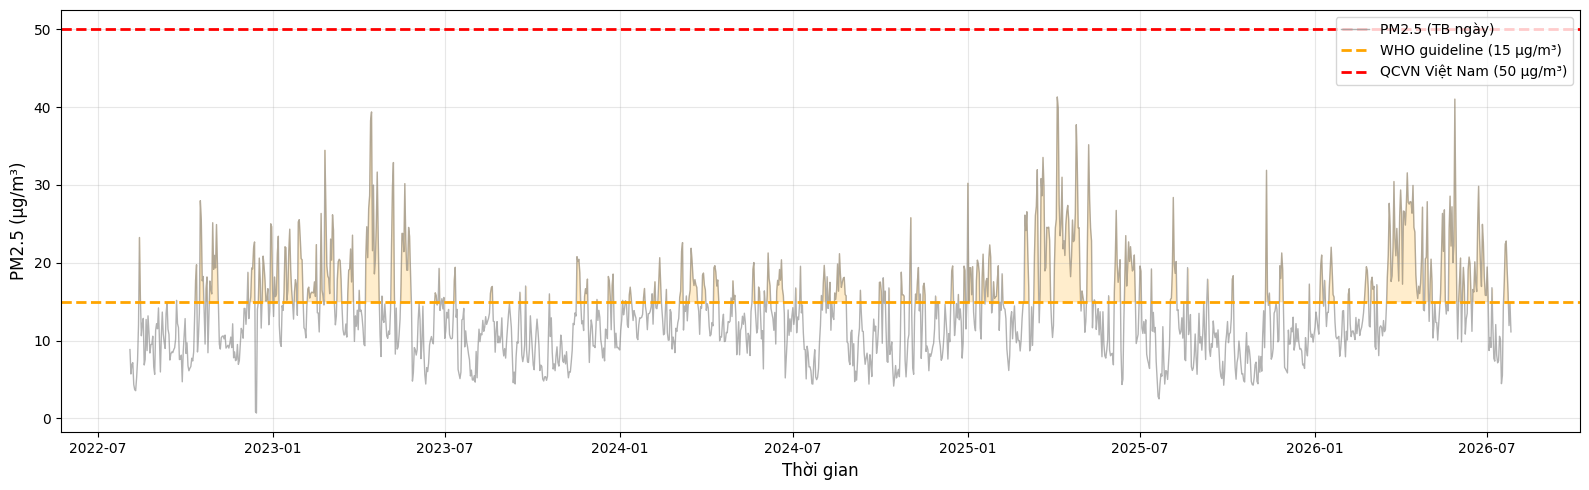
\includegraphics[width=\textwidth]{figures/pm25_who_qcvn.png}
\caption{PM2.5 trung bình ngày so với ngưỡng khuyến nghị WHO và QCVN Việt Nam}
\label{fig:whoqcvn}
\end{figure}

Trong tổng số 1.453 ngày có dữ liệu, có \textbf{510 ngày (35.1\%)} có nồng độ PM2.5 trung bình 24h vượt ngưỡng khuyến nghị của WHO Air Quality Guideline 2021 (15~$\mu$g/m$^3$) — cho thấy hơn một phần ba số ngày trong giai đoạn quan sát không đạt chuẩn an toàn theo khuyến nghị quốc tế. Ngược lại, \textbf{không có ngày nào (0.0\%)} vượt ngưỡng QCVN 05:2013/BTNMT của Việt Nam (50~$\mu$g/m$^3$) (Hình~\ref{fig:whoqcvn}) — phản ánh khoảng cách đáng kể giữa quy chuẩn hiện hành trong nước và chuẩn khuyến nghị siết chặt hơn của WHO.

\subsection*{Biến động PM2.5 theo mùa trong năm}

\begin{figure}[H]
\centering
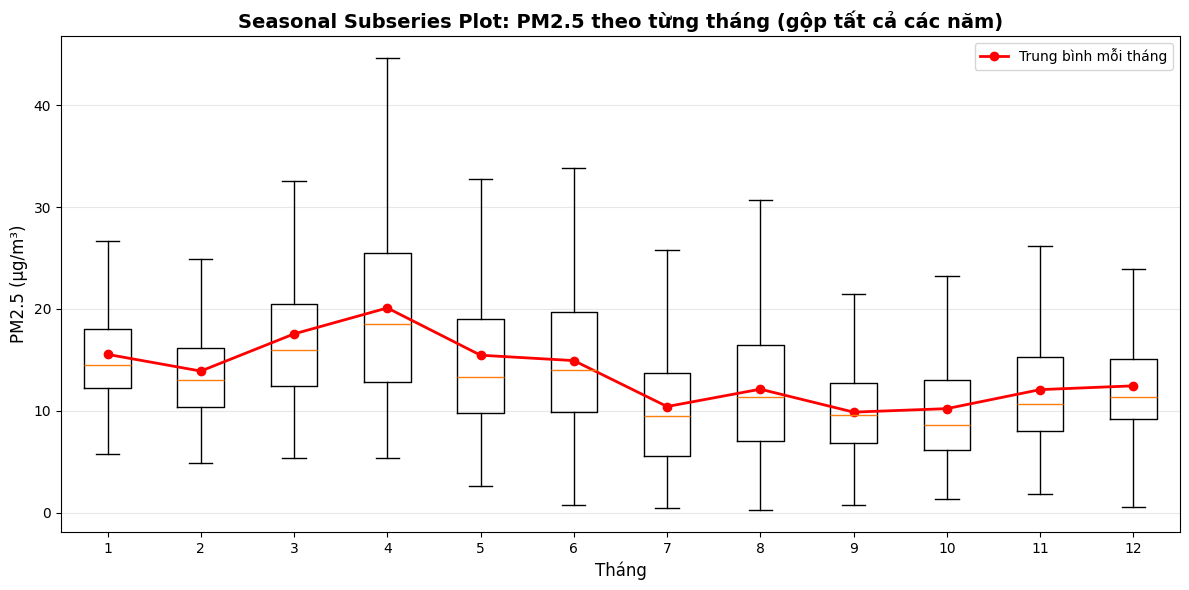
\includegraphics[width=0.85\textwidth]{figures/pm25_seasonal_subseries.png}
\caption{Seasonal Subseries Plot: PM2.5 theo từng tháng (gộp tất cả các năm)}
\label{fig:seasonal}
\end{figure}

Hình~\ref{fig:seasonal} cho thấy PM2.5 đạt đỉnh vào các tháng 1--4 (cao nhất ở tháng 4, trung bình $\approx$20~$\mu$g/m$^3$), giảm dần xuống mức thấp nhất vào các tháng 7--10 (trung bình $\approx$10--12~$\mu$g/m$^3$), rồi tăng nhẹ trở lại vào tháng 11--12. Kiểu biến động này phù hợp với đặc trưng khí hậu khu vực Nam Trung Bộ: các tháng đầu năm (gió mùa Đông Bắc, ít mưa) khiến bụi mịn tích tụ nhiều hơn, trong khi mùa mưa (tháng 7--10) giúp rửa trôi các hạt lơ lửng, làm giảm nồng độ PM2.5. Kết quả này nhất quán với nhận xét ở Mục~2.5 rằng giai đoạn dữ liệu mới (cuối tháng 7 -- tháng 8/2026, mùa mưa) có PM2.5 thấp và ít biến động hơn.

% ==================== 2.3 TIỀN XỬ LÝ ====================
\section{Tiền xử lý dữ liệu}

\subsection*{Loại bỏ đặc trưng không liên quan}

Dựa trên kết quả phân tích tương quan ở Mục~2.2 (Correlation Heatmap $|r| < 0.1$, và Cross-Correlation Function ở mọi độ trễ đều $< 0.16$), ba biến \textbf{Dust}, \textbf{UV Index}, \textbf{UV Index Clear Sky} được loại bỏ khỏi tập đặc trưng đầu vào nhằm giảm nhiễu và số chiều dữ liệu.

\subsection*{Feature Engineering: Mã hóa chu kỳ thời gian}

Hai đặc trưng thời gian rời rạc \textbf{hour} và \textbf{month} được mã hóa dạng \textbf{cyclical encoding} bằng cặp hàm sin/cos, nhằm tránh điểm gãy giả tạo (ví dụ 23h và 0h về bản chất "gần nhau" chứ không "cách xa 23 đơn vị" như khi giữ nguyên dạng số nguyên):

\begin{equation}
\text{hour\_sin} = \sin\!\left(\frac{2\pi \cdot \text{hour}}{24}\right), \qquad
\text{hour\_cos} = \cos\!\left(\frac{2\pi \cdot \text{hour}}{24}\right)
\end{equation}
\begin{equation}
\text{month\_sin} = \sin\!\left(\frac{2\pi \cdot \text{month}}{12}\right), \qquad
\text{month\_cos} = \cos\!\left(\frac{2\pi \cdot \text{month}}{12}\right)
\end{equation}

Hai biến \textbf{day} và \textbf{year} bị loại bỏ: \textit{day} (ngày trong tháng) không có chu kỳ vật lý rõ ràng liên quan đến PM2.5, còn \textit{year} là giá trị tuyệt đối không tổng quát hóa được cho các thời điểm tương lai nằm ngoài phạm vi dữ liệu huấn luyện.

\subsection*{Chia tập Train / Validation / Test theo thời gian}

Do bản chất tuần tự của dữ liệu, việc chia tập không được thực hiện ngẫu nhiên (shuffle) như bài toán học có giám sát thông thường, để tránh rò rỉ dữ liệu (data leakage) từ tương lai vào quá khứ. Dữ liệu được chia theo mốc thời gian với tỷ lệ 70/15/15:

\begin{table}[H]
\centering
\caption{Phân chia tập Train / Validation / Test theo thời gian}
\begin{tabular}{lrll}
\toprule
Tập & Số dòng & Từ & Đến \\
\midrule
Train & 24.405 & 2022-08-04 07:00 & 2025-05-17 03:00 \\
Validation & 5.230 & 2025-05-17 04:00 & 2025-12-21 01:00 \\
Test & 5.230 & 2025-12-21 02:00 & 2026-07-26 23:00 \\
\bottomrule
\end{tabular}
\end{table}

\subsection*{Chuẩn hóa dữ liệu}

Toàn bộ đặc trưng số được chuẩn hóa về khoảng $[0,1]$ bằng \textbf{MinMaxScaler}. Điểm quan trọng cần lưu ý: scaler chỉ được \textit{fit} trên tập Train, sau đó dùng để \textit{transform} tập Validation và Test — nhằm tránh rò rỉ thông tin thống kê (min/max) của tập validation/test vào quá trình huấn luyện.

\subsection*{Sliding Window: Tạo cặp \texorpdfstring{$(X, y)$}{(X, y)}}

Từ dữ liệu đã chuẩn hóa, các cặp $(X, y)$ được tạo bằng kỹ thuật sliding window (Mục~1.1) với horizon $= 1$. Với mỗi vị trí $i$, $X_i$ là ma trận gồm \texttt{window\_size} bước thời gian $\times$ 11 đặc trưng, và $y_i$ là giá trị PM2.5 tại bước kế tiếp.

% ==================== 2.4 XÂY DỰNG MÔ HÌNH ====================
\section{Xây dựng mô hình}

\subsection*{Kiến trúc GRU triển khai}

Mô hình được cài đặt bằng PyTorch, gồm một khối GRU 2 lớp (\texttt{num\_layers=2}) với dropout $0.2$ giữa các lớp, theo sau bởi một lớp fully-connected tuyến tính ánh xạ trạng thái ẩn tại bước thời gian cuối cùng thành giá trị PM2.5 dự báo (Hình mô tả kiến trúc — xem công thức Mục~1.4). Với \texttt{hidden\_size=64} và 11 đặc trưng đầu vào, mô hình có tổng cộng \textbf{39.809 tham số có thể huấn luyện}.

\subsection*{Tinh chỉnh siêu tham số}

Grid Search được thực hiện trên không gian ba siêu tham số: \texttt{window\_size} $\in \{24, 48\}$ giờ, \texttt{hidden\_size} $\in \{32, 64\}$, \texttt{learning\_rate} $\in \{0.001, 0.0005\}$ — mỗi cấu hình huấn luyện tối đa 6 epoch với early stopping (patience$=2$), đánh giá bằng validation loss (MAE, thang chuẩn hóa).

\begin{table}[H]
\centering
\caption{Kết quả Grid Search siêu tham số (sắp xếp theo validation loss)}
\begin{tabular}{rrrr}
\toprule
window\_size (h) & hidden\_size & learning\_rate & val\_loss (MAE, scaled) \\
\midrule
48 & 64 & 0.001  & 0.01276 \\
24 & 64 & 0.001  & 0.01390 \\
48 & 32 & 0.001  & 0.01410 \\
24 & 32 & 0.001  & 0.01431 \\
24 & 64 & 0.0005 & 0.01502 \\
48 & 64 & 0.0005 & 0.01738 \\
24 & 32 & 0.0005 & 0.01801 \\
48 & 32 & 0.0005 & 0.01852 \\
\bottomrule
\end{tabular}
\end{table}

\begin{sloppypar}
Cấu hình có validation loss thấp nhất tuyệt đối là \texttt{window=48h, hidden=64, lr=0.001} (0.01276). Tuy nhiên, để tránh chọn một mô hình phức tạp/tốn chi phí tính toán hơn chỉ vì một khác biệt nhỏ không đáng kể, tiêu chí lựa chọn cuối cùng là: trong số các cấu hình có validation loss nằm trong khoảng 10\% so với giá trị tốt nhất, chọn cấu hình có chi phí tính toán thấp nhất (ước lượng bằng $\text{window\_size} \times \text{hidden\_size}$). Theo tiêu chí này, cấu hình được chọn là:
\end{sloppypar}

\[
\texttt{window\_size} = 24\text{h}, \quad \texttt{hidden\_size} = 64, \quad \texttt{learning\_rate} = 0.001
\]

Cửa sổ 24 giờ cũng phù hợp với phát hiện từ ACF (Hình~\ref{fig:acfpacf}): chu kỳ ngày là chu kỳ chi phối hành vi ngắn hạn của PM2.5, nên một cửa sổ dài hơn (48h) không mang lại cải thiện tương xứng với chi phí tính toán tăng thêm.

\subsection*{Huấn luyện mô hình cuối cùng}

Với cấu hình đã chọn, mô hình được huấn luyện lại với ngân sách epoch lớn hơn (tối đa 25 epoch, patience$=5$) để hội tụ đầy đủ hơn.

\begin{figure}[H]
\centering
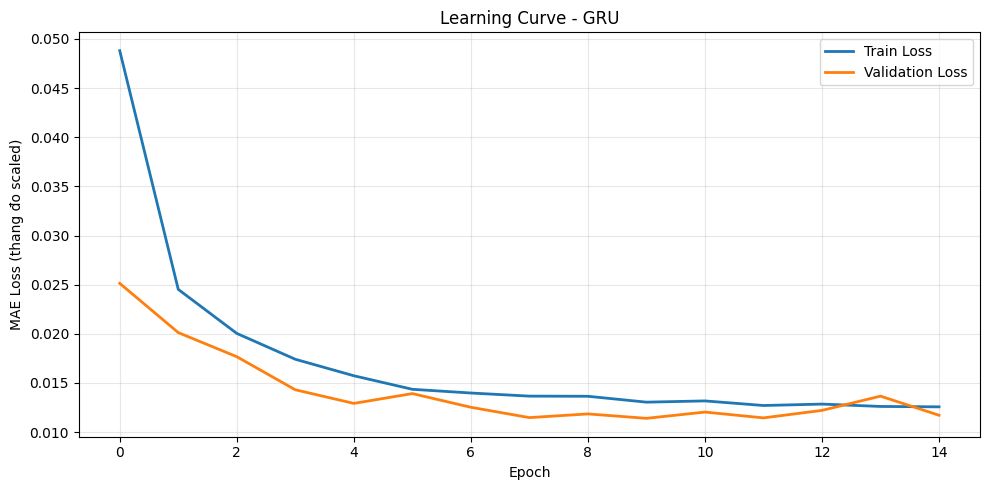
\includegraphics[width=0.75\textwidth]{figures/learning_curve.png}
\caption{Learning curve — GRU (window=24h, hidden=64)}
\label{fig:learning_curve}
\end{figure}

Quá trình huấn luyện dừng sớm ở epoch 15 (val\_loss tốt nhất đạt được ở epoch 10, $\approx 0.0114$), cho thấy early stopping hoạt động hiệu quả trong việc ngăn mô hình overfit lên tập train sau khi đã hội tụ trên tập validation (Hình~\ref{fig:learning_curve}).

\subsection*{Đánh giá trên tập Test}

Mô hình GRU (window=24h, hidden\_size=64) được đánh giá trên toàn bộ tập Test bằng hai chỉ số MAE và RMSE (thang đo gốc, $\mu$g/m$^3$).

\begin{table}[H]
\centering
\caption{Hiệu năng mô hình GRU trên tập Test (thang đo gốc, $\mu$g/m$^3$)}
\begin{tabular}{lrr}
\toprule
Mô hình & MAE ($\mu$g/m$^3$) & RMSE ($\mu$g/m$^3$) \\
\midrule
\textbf{GRU (window=24h)} & \textbf{1.172} & \textbf{2.173} \\
\bottomrule
\end{tabular}
\end{table}

\begin{figure}[H]
\centering
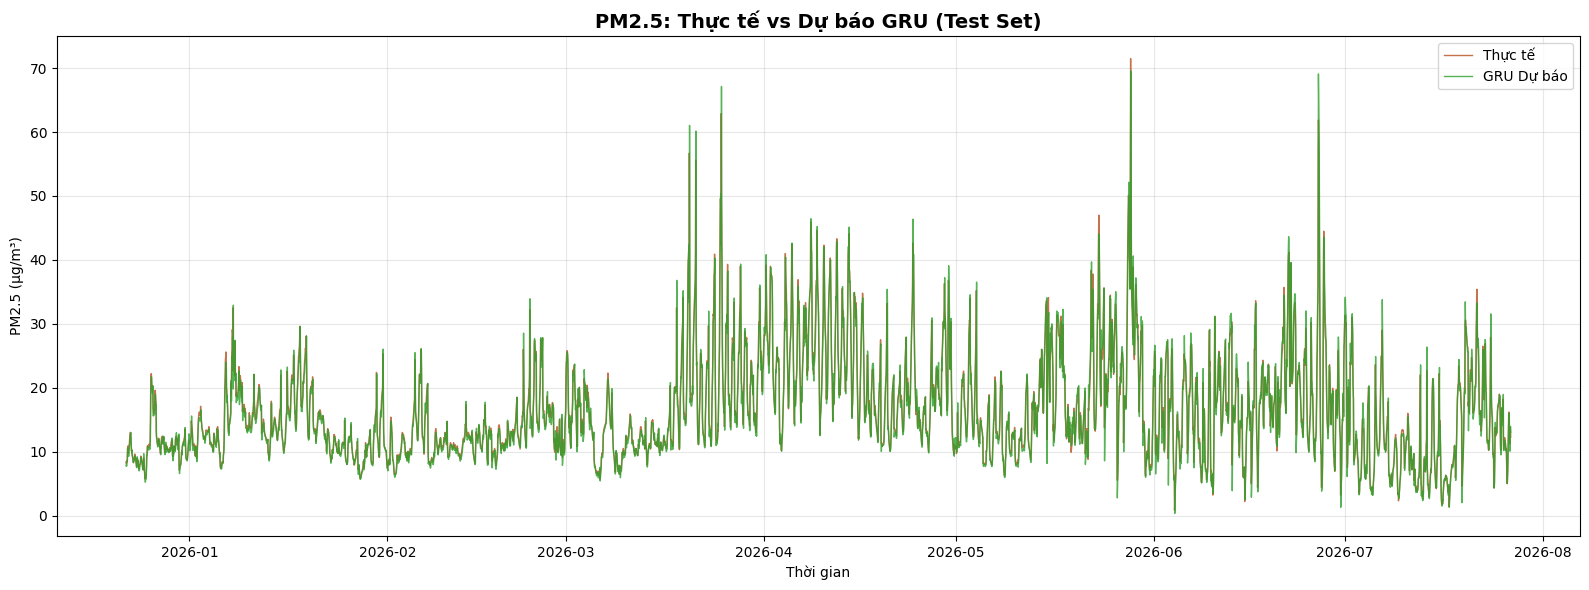
\includegraphics[width=\textwidth]{figures/prediction_test.png}
\caption{PM2.5: Thực tế và Dự báo GRU trên tập Test}
\label{fig:pred_test}
\end{figure}

Với MAE $=1.172\,\mu$g/m$^3$ trên thang đo gốc — chỉ tương đương khoảng $8.5\%$ so với giá trị trung bình PM2.5 của toàn bộ dữ liệu ($13.73\,\mu$g/m$^3$, xem Bảng~\ref{tab:describe}) — mô hình cho sai số tương đối nhỏ. Hình~\ref{fig:pred_test} cho thấy đường dự báo GRU (xanh lá) bám khá sát đường thực tế (cam) trên toàn bộ tập Test, kể cả tại các đợt tăng đột biến.

\subsection*{Phân tích Residual}

\begin{figure}[H]
\centering
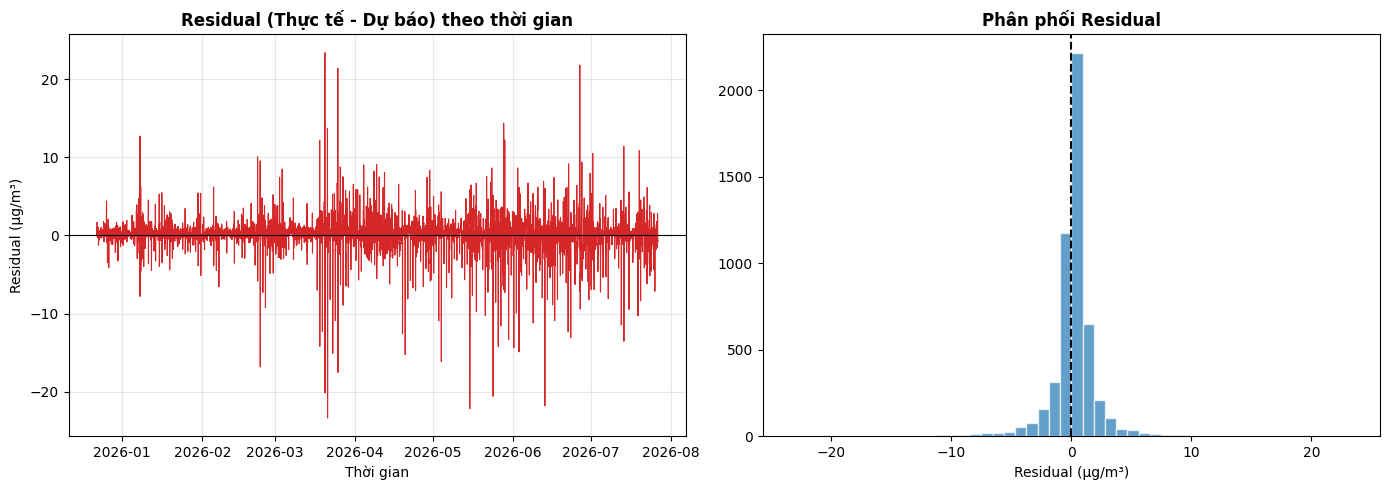
\includegraphics[width=\textwidth]{figures/residual_test.png}
\caption{Residual (Thực tế $-$ Dự báo) trên tập Test}
\label{fig:resid_test}
\end{figure}

Residual trên tập Test có \textbf{mean $= 0.175\,\mu$g/m$^3$}, \textbf{std $= 2.166\,\mu$g/m$^3$} — mean gần 0 cho thấy mô hình không thiên lệch (bias) hệ thống theo một hướng cụ thể. Phân phối residual (Hình~\ref{fig:resid_test}) tập trung quanh 0, tuy vẫn còn một số giá trị residual lớn tương ứng với các thời điểm PM2.5 tăng đột biến khó dự báo — đây là hạn chế phổ biến của các mô hình dự báo chuỗi thời gian khi đối mặt với sự kiện hiếm/bất thường.

% ==================== 2.5 ĐÁNH GIÁ OUT-OF-SAMPLE ====================
\section{Đánh giá trên dữ liệu mới (Out-of-sample)}

Một điểm mạnh trong thiết kế thực nghiệm của tiểu luận này là việc đánh giá mô hình không chỉ dừng lại ở tập Test (vốn vẫn nằm trong cùng khoảng thời gian thu thập dữ liệu ban đầu), mà còn được kiểm chứng trên một bộ dữ liệu \textbf{hoàn toàn mới}, được thu thập ở một thời điểm sau đó — mô phỏng sát tình huống triển khai thực tế khi mô hình phải dự báo cho dữ liệu chưa từng "nhìn thấy" trong suốt quá trình phát triển.

\subsection*{Thu thập và xử lý dữ liệu mới}

Bộ dữ liệu mới (\texttt{new\_data.csv}) gồm \textbf{696 dòng}, từ \texttt{2026-07-27 00:00} đến \texttt{2026-08-24 23:00} (29 ngày), được thu thập từ cùng nguồn Open-Meteo API tại cùng vị trí. Dữ liệu được làm sạch và tiền xử lý theo đúng quy trình đã áp dụng ở Mục~2.1--2.3 (cùng scaler đã fit trên tập Train trước đó — \textbf{không fit lại} để đảm bảo tính nhất quán và tránh leakage). Để có đủ ngữ cảnh (context) cho các điểm dự báo đầu tiên của dữ liệu mới, 24 giờ cuối của tập Test được nối thêm vào trước dữ liệu mới làm phần lịch sử — toàn bộ phần ngữ cảnh này đều là dữ liệu \textit{quá khứ} so với từng điểm cần dự báo, nên không phát sinh rò rỉ dữ liệu.

\subsection*{Kết quả dự báo}

\begin{table}[H]
\centering
\caption{Hiệu năng mô hình GRU trên dữ liệu mới (out-of-sample, $\mu$g/m$^3$)}
\begin{tabular}{lrr}
\toprule
Mô hình & MAE ($\mu$g/m$^3$) & RMSE ($\mu$g/m$^3$) \\
\midrule
\textbf{GRU (window=24h)} & \textbf{0.769} & \textbf{1.366} \\
\bottomrule
\end{tabular}
\end{table}

\begin{figure}[H]
\centering
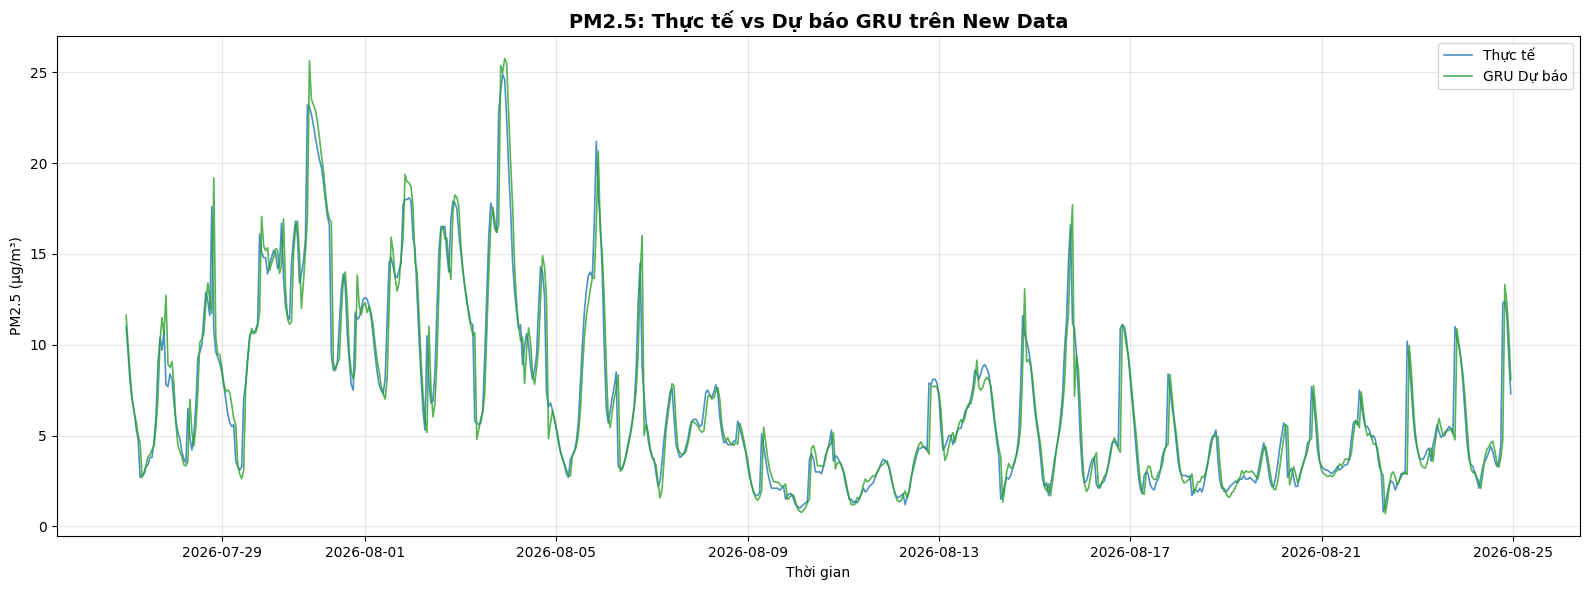
\includegraphics[width=\textwidth]{figures/prediction_newdata.png}
\caption{PM2.5: Thực tế và Dự báo GRU trên dữ liệu mới}
\label{fig:pred_new}
\end{figure}

Đáng chú ý, sai số tuyệt đối trên dữ liệu mới (MAE $=0.769\,\mu$g/m$^3$) thấp hơn cả sai số trên tập Test (MAE $=1.172\,\mu$g/m$^3$) — điều này phù hợp với thực tế nồng độ PM2.5 trong giai đoạn cuối tháng 7 -- tháng 8/2026 (mùa mưa tại khu vực Nam Trung Bộ) nhìn chung thấp và ít biến động đột biến hơn giai đoạn tập Test, khiến bài toán dự báo trở nên "dễ" hơn tương đối trong giai đoạn này.

\subsection*{Phân tích Residual trên dữ liệu mới}

\begin{figure}[H]
\centering
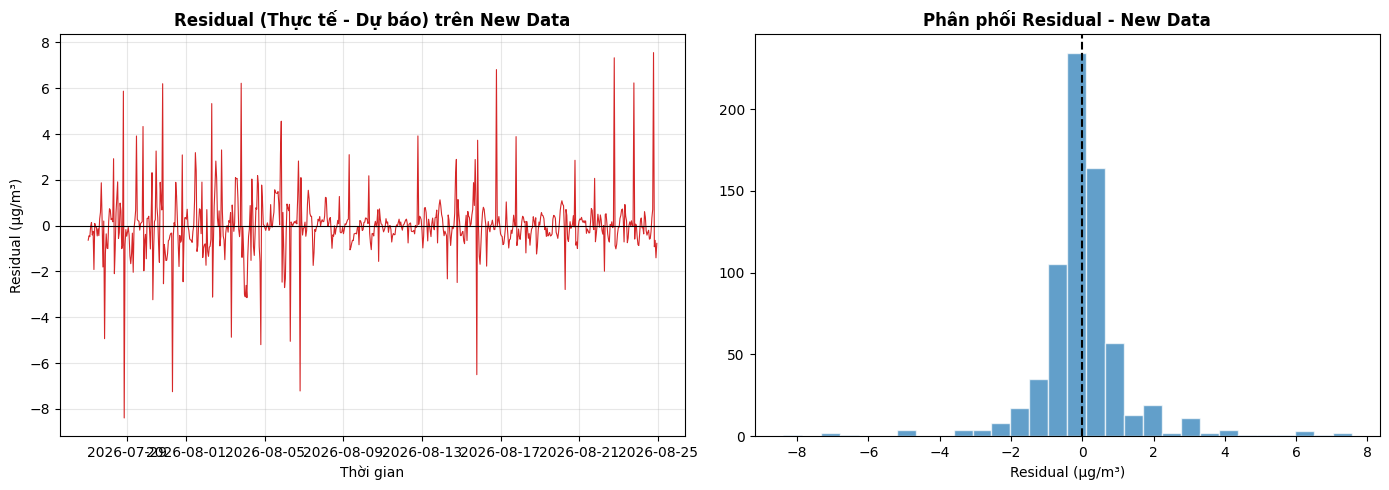
\includegraphics[width=\textwidth]{figures/residual_newdata.png}
\caption{Residual (Thực tế $-$ Dự báo) trên dữ liệu mới}
\label{fig:resid_new}
\end{figure}

\begin{sloppypar}
Residual trên dữ liệu mới có \textbf{mean $= 0.013\,\mu$g/m$^3$} (gần như bằng 0) và \textbf{std $= 1.366\,\mu$g/m$^3$} — thấp hơn cả độ lệch chuẩn residual trên tập Test, củng cố kết luận rằng mô hình duy trì được khả năng tổng quát hóa tốt khi triển khai trên dữ liệu thực sự mới, không có dấu hiệu suy giảm hiệu năng (model drift) đáng kể trong giai đoạn quan sát.
\end{sloppypar}

% ==================== 2.6 MULTI-STEP FORECASTING ====================
\section{Mở rộng: Dự báo đa bước (Multi-step Forecasting)}

Mô hình ở Mục~2.4 chỉ dự báo được đúng \textbf{1 giờ tới} (horizon $h=1$) — như đã phân tích ở Mục~1.4, đây gần như chỉ mang tính "nowcasting", chưa đủ lead time để cảnh báo/hành động trước. Phần này thử nghiệm mở rộng sang dự báo \textbf{$H=6$ giờ tới}, áp dụng đúng hai chiến lược đã trình bày lý thuyết ở Mục~1.4: \textbf{Recursive GRU} và \textbf{Direct GRU}.

\subsection*{Recursive GRU: tái sử dụng model horizon=1}

Tái sử dụng nguyên model GRU (window=24h, hidden\_size=64) đã huấn luyện ở Mục~2.4 — \textbf{không huấn luyện lại}. Model được gọi lặp lại 6 lần theo đúng cơ chế đã mô tả ở Hình~\ref{fig:recursive}: PM2.5 dự đoán ở bước trước được đưa ngược vào cửa sổ cho bước sau, các đặc trưng ngoại sinh dùng persistence, đặc trưng lịch tính chính xác cho từng giờ tương lai.

\subsection*{Direct GRU: Grid Search và huấn luyện riêng}

Vì Direct GRU là một model hoàn toàn mới (đổi lớp fully-connected cuối thành $\text{Linear}(\text{hidden}, 6)$ — xem Hình~\ref{fig:direct}), một Grid Search riêng được thực hiện trên cùng không gian siêu tham số đã dùng ở Mục~2.4.2 (\texttt{window\_size} $\in \{24, 48\}$, \texttt{hidden\_size} $\in \{32, 64\}$, \texttt{learning\_rate} $\in \{0.001, 0.0005\}$), theo cùng tiêu chí chọn cấu hình (10\% dung sai + chi phí tính toán thấp nhất). Cấu hình được chọn là \texttt{window\_size=24h, hidden\_size=32, learning\_rate=0.001} — nhẹ hơn model horizon=1 gốc (hidden\_size=32 thay vì 64).

\subsection*{So sánh trên tập Test}

\begin{table}[H]
\centering
\caption{So sánh MAE/RMSE giữa Recursive GRU và Direct GRU theo từng bước horizon (5.201 mốc gốc chung)}
\begin{tabular}{rrrrrr}
\toprule
Horizon $h$ & Recursive MAE & Direct MAE & Recursive RMSE & Direct RMSE & Direct tốt hơn (\%) \\
\midrule
1 & 1.172 & 1.210 & 2.174 & 2.182 & $-3.2$ \\
2 & 2.140 & 1.951 & 3.483 & 3.198 & $8.8$ \\
3 & 2.988 & 2.576 & 4.613 & 3.972 & $13.8$ \\
4 & 3.715 & 3.029 & 5.576 & 4.511 & $18.5$ \\
5 & 4.341 & 3.401 & 6.383 & 4.956 & $21.7$ \\
6 & 4.880 & 3.683 & 7.075 & 5.274 & $24.5$ \\
\bottomrule
\end{tabular}
\end{table}

\begin{figure}[H]
\centering
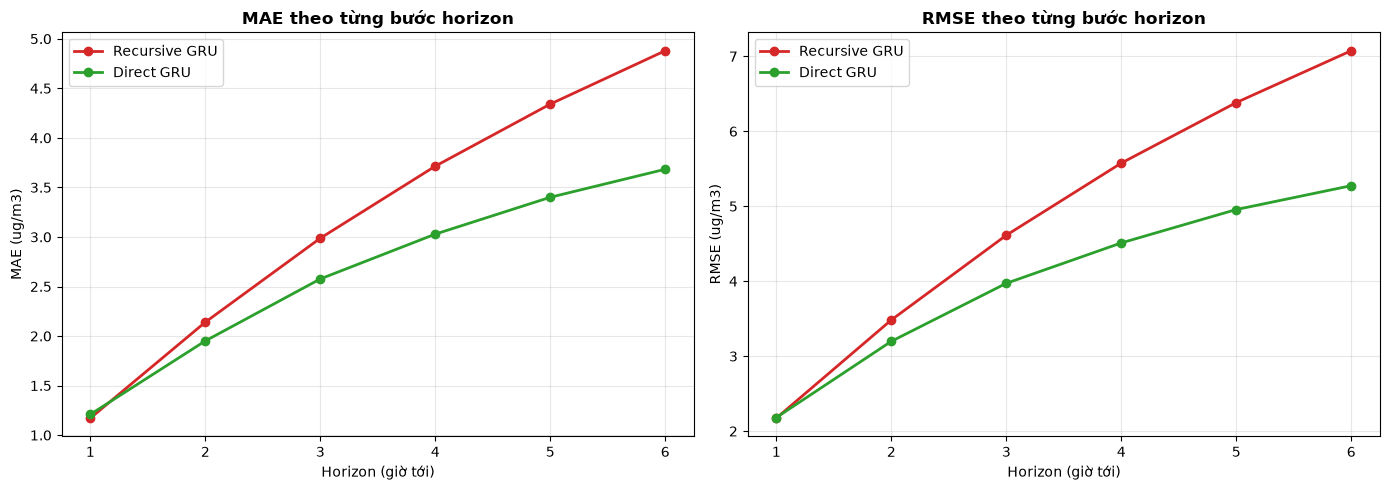
\includegraphics[width=\textwidth]{figures/multistep_comparison.png}
\caption{MAE và RMSE của Recursive GRU và Direct GRU theo từng bước horizon}
\label{fig:ms_comparison}
\end{figure}

Hình~\ref{fig:ms_comparison} cho thấy rõ hiện tượng \textbf{dồn sai số} (error compounding) của Recursive GRU đã dự đoán ở Mục~1.4: ở $h=1$, Recursive thậm chí nhỉnh hơn Direct một chút ($-3.2\%$, vì đây chính xác là model chuyên biệt horizon=1 đã được Grid Search kỹ ở Mục~2.4). Nhưng từ $h=2$ trở đi, Direct GRU vượt trội rõ rệt và khoảng cách ngày càng giãn ra — đến $h=6$, Direct tốt hơn Recursive tới $24.5\%$ về MAE.

\begin{figure}[H]
\centering
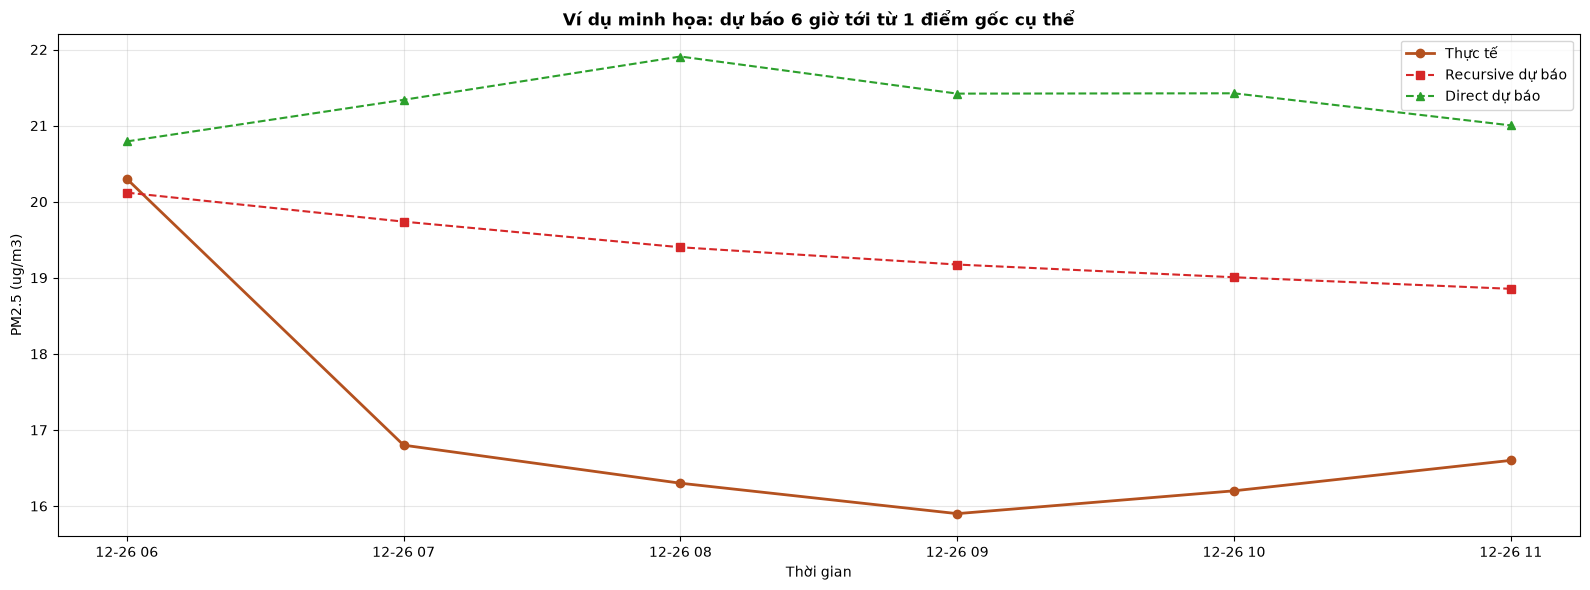
\includegraphics[width=\textwidth]{figures/multistep_example.png}
\caption{Ví dụ minh họa dự báo 6 giờ tới từ một điểm gốc cụ thể trong tập Test}
\label{fig:ms_example}
\end{figure}

\subsection*{Phân tích Residual}

\begin{figure}[H]
\centering
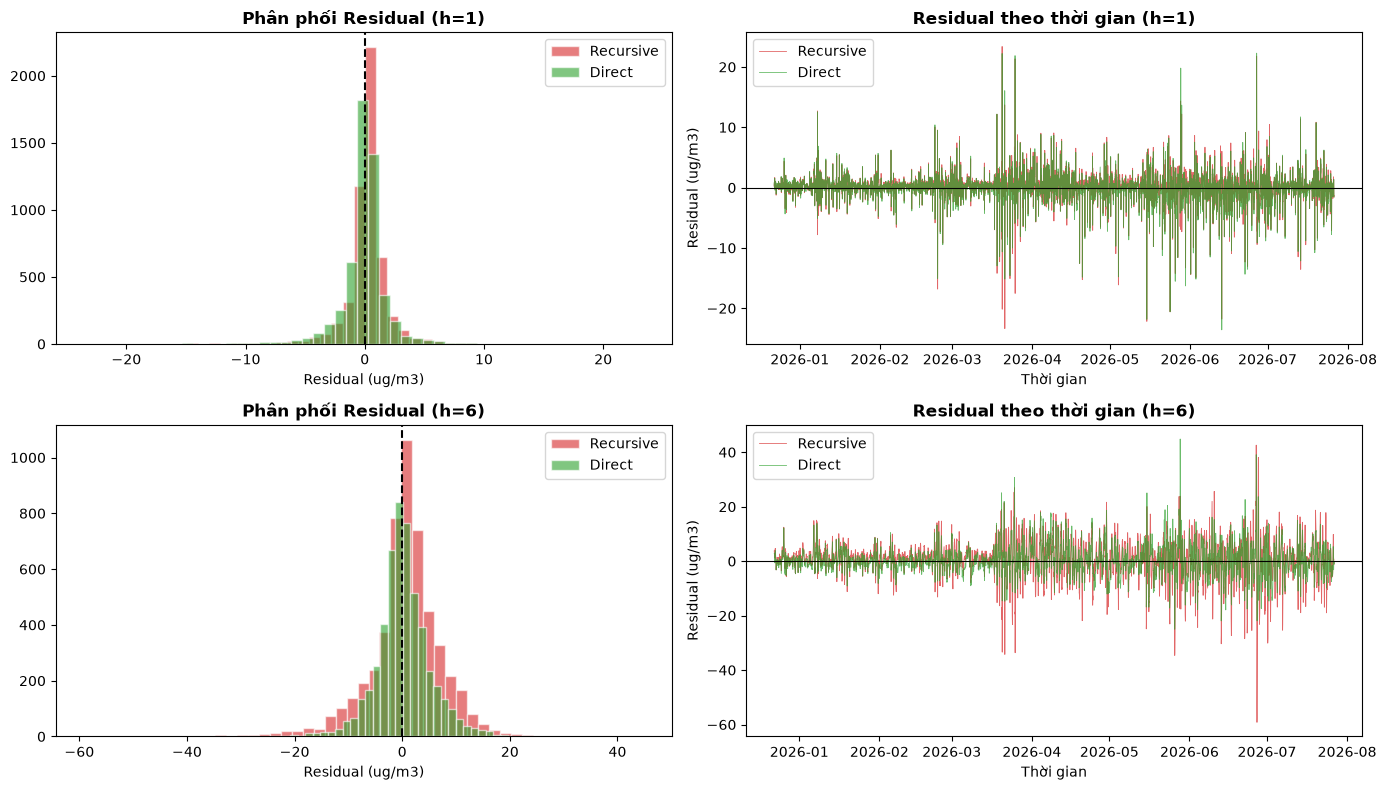
\includegraphics[width=\textwidth]{figures/multistep_residual.png}
\caption{Phân phối và diễn biến Residual của Recursive GRU và Direct GRU tại $h=1$ và $h=6$}
\label{fig:ms_residual}
\end{figure}

Tại $h=1$, độ lệch chuẩn residual của hai model gần tương đương nhau (Recursive: mean$=0.175$, std$=2.167\,\mu$g/m$^3$; Direct: mean$=-0.042$, std$=2.181\,\mu$g/m$^3$). Nhưng tại $h=6$, độ phân tán của Recursive tăng nhanh hơn hẳn (std$=7.046\,\mu$g/m$^3$) so với Direct (std$=5.265\,\mu$g/m$^3$) — Hình~\ref{fig:ms_residual} cho thấy trực quan phân phối residual của Recursive bị "loe" rộng hơn đáng kể ở $h=6$, xác nhận bằng thực nghiệm cơ chế dồn sai số đã lý giải bằng lý thuyết ở Mục~1.4.

% ==================== 2.7 KẾT LUẬN ====================
\section{Kết luận}

Trong tiểu luận này, bài toán dự báo nồng độ PM2.5 theo chuỗi thời gian tại thành phố Quy Nhơn đã được xây dựng và đánh giá thông qua mô hình mạng GRU. Quy trình thực hiện đầy đủ các bước: làm sạch dữ liệu, phân tích khám phá chuyên biệt cho chuỗi thời gian (kiểm định tính dừng ADF/KPSS, xu hướng Mann-Kendall, tính chu kỳ qua ACF/PACF/Periodogram/Decomposition), tiền xử lý và feature engineering, tinh chỉnh siêu tham số bằng Grid Search, và đánh giá mô hình.

Kết quả cho thấy mô hình GRU (window=24h, hidden\_size=64) đạt MAE $=1.172\,\mu$g/m$^3$ trên tập Test — tương đương khoảng $8.5\%$ so với giá trị trung bình PM2.5 của toàn bộ dữ liệu. Đặc biệt, khi kiểm chứng trên một bộ dữ liệu hoàn toàn mới được thu thập ở giai đoạn sau đó, mô hình vẫn duy trì hiệu năng tốt (MAE $=0.769\,\mu$g/m$^3$), với residual gần như không thiên lệch — chứng tỏ khả năng tổng quát hóa của mô hình không chỉ dừng lại ở một tập hold-out tĩnh mà còn giữ vững khi đối mặt với dữ liệu thực sự chưa từng biết trước.

Mục~2.6 mở rộng thêm bài toán sang dự báo đa bước ($H=6$ giờ), so sánh hai chiến lược \textbf{Recursive} (tái sử dụng model horizon=1, không train lại) và \textbf{Direct} (model mới, Grid Search riêng). Kết quả cho thấy Direct GRU vượt trội rõ rệt so với Recursive từ $h=2$ trở đi (tốt hơn tới $24.5\%$ về MAE ở $h=6$), xác nhận bằng thực nghiệm hiện tượng dồn sai số (error compounding) đã lý giải bằng lý thuyết ở Mục~1.4 — trong khi ở $h=1$, hai chiến lược cho kết quả gần tương đương.

Bên cạnh những kết quả tích cực, tiểu luận còn một số hạn chế: (1) dữ liệu chỉ trải dài khoảng 4 năm, giới hạn khả năng học đầy đủ chu kỳ năm mà Periodogram đã chỉ ra là chu kỳ chiếm ưu thế; (2) dù đã thử nghiệm mở rộng multi-step, độ chính xác dự báo vẫn suy giảm khá nhanh theo horizon — ngay cả Direct (không dồn sai số) cũng giảm đáng kể từ $h=1$ đến $h=6$, cho thấy còn nhiều dư địa cải thiện cho bài toán dự báo xa; (3) các kiến trúc GRU dạng Encoder-only (horizon=1, Direct) là những kiến trúc duy nhất được thử nghiệm thực tế, chưa so sánh với LSTM, Temporal Convolutional Network, Transformer, hay kiến trúc Seq2seq (Encoder–Decoder) đầy đủ — kiến trúc mà GRU vốn được thiết kế nguyên bản để giải quyết.

Hướng phát triển tiếp theo có thể tập trung vào: cài đặt kiến trúc Seq2seq (Encoder–Decoder) đầy đủ cho bài toán multi-step; mở rộng horizon dự báo xa hơn 6 giờ; thay giả định persistence của Recursive bằng dự báo thực sự cho các đặc trưng ngoại sinh (ví dụ dự báo thời tiết từ mô hình khí tượng số); và thử nghiệm thêm các kiến trúc/hàm mất mát khác để đánh giá khả năng cải thiện thêm hiệu năng mô hình.

% ==================== TÀI LIỆU THAM KHẢO ====================
\chapter*{Tài liệu tham khảo}
\addcontentsline{toc}{chapter}{Tài liệu tham khảo}

\textit{(Danh sách tài liệu tham khảo sẽ được bổ sung.)}

\end{document}
